% This is samplepaper.tex, a sample chapter demonstrating the
% LLNCS macro package for Springer Computer Science proceedings;
% Version 2.21 of 2022/01/12
%
\documentclass[runningheads]{llncs}
%
\usepackage[T1]{fontenc}
% T1 fonts will be used to generate the final print and online PDFs,
% so please use T1 fonts in your manuscript whenever possible.
% Other font encondings may result in incorrect characters.
%
\usepackage{graphicx}
% Used for displaying a sample figure. If possible, figure files should
% be included in EPS format.
%
% If you use the hyperref package, please uncomment the following two lines
% to display URLs in blue roman font according to Springer's eBook style:
%\usepackage{color}
%\renewcommand\UrlFont{\color{blue}\rmfamily}
%\urlstyle{rm}
%


% \usepackage{setspace}
%\AtBeginDocument{\setstretch{.9}}
%\doublespacing  % doublespacing is done after title and before abstract

\usepackage{caption}
\usepackage{subcaption}
\usepackage[title]{appendix}

\usepackage[margin=1.2in]{geometry}

%\usepackage{lineno}
%\linenumbers

% \usepackage{fullpage}
\usepackage{authblk}
\usepackage[utf8]{inputenc}
\usepackage{amsmath,bm}
\usepackage{amsthm}
\usepackage{amssymb}
\usepackage{hyperref}
\usepackage{adjustbox}
\usepackage{multirow}
\usepackage{graphicx}
\usepackage{booktabs}
\usepackage{caption}
\usepackage{subcaption}
\usepackage[table]{xcolor}
\usepackage{tabu}
\usepackage{subcaption}
\usepackage{longtable}
\usepackage{amssymb}
\usepackage{footnote}
\usepackage{hyperref}
\usepackage{multirow}
\usepackage{comment}
\usepackage{cite}
\usepackage{threeparttable}
\usepackage{makecell}
\usepackage{mathtools} % for multiline-multicase equation
\usepackage{float}
\usepackage{array}
\usepackage{tabularx} % in the preamble
\usepackage{tikz}
\usepackage{ulem}
\usepackage{algorithm2e}

\usepackage{tabularx}
\newcolumntype{Y}{>{\centering\arraybackslash}X}
\newcolumntype{C}[1]{>{\centering\arraybackslash}m{#1}}

\usepackage{xcolor}
\newcommand{\add}[1]{{\color{blue} #1}}
\newcommand{\addb}[1]{{\color{red} #1}}
\newcommand{\SR}[1]{{\color{red} #1}}
\newcommand{\methodname}{{\color{purple}Method\_Name~}}

\newtheorem{theorem}{Theorem}[section]
\newtheorem{corollary}{Corollary}[theorem]
\newtheorem{lemma}[theorem]{Lemma}

% \renewcommand{\thetheorem}{\arabic{theorem}}  % to start numbering from 1

%\usepackage{booktabs, caption, makecell}
%\renewcommand\theadfont{\bfseries}
\usepackage{subfiles} % For subfiles
\usepackage{hyperref}
\usepackage[labelfont=bf]{caption}

\usepackage{xcolor}

\newcommand{\add}[1]{{\color{blue} #1}}
\newcommand{\addr}[1]{{\color{red} #1}}

\renewcommand\theadalign{bc}
\renewcommand\theadfont{\bfseries}
\renewcommand\theadgape{\Gape[4pt]}
\renewcommand\cellgape{\Gape[4pt]}

\makesavenoteenv{tabular}
\makesavenoteenv{table}

\hypersetup{
    urlcolor=blue,
}

\begin{document}
%
\title{STELAR-X: Scaling STELAR for Triplet Based Inference of Ultra-large Phylogentic Trees}



%Pushing the Boundaries of Phylogenomic Scale: STELAR-X Enables Coalescent-Based Species Tree Inference for 50,000 Species

%Ultra-Large and Statistically Consistent Species Tree Inference: STELAR-X Scales to 50,000 Species

%STELAR-X: Scaling Coalescent-Based Species Tree Inference to 50,000 Species and Beyond

% %
% \titlerunning{QT-WEAVER}
% % If the paper title is too long for the running head, you can set
% % an abbreviated paper title here
% %
% \author{Navid Bin Hasan\inst{1,\dag}\orcidID{0009-0004-7792-9798} \and
% Sohaib\inst{1,\dag}\orcidID{0009-0003-8861-4743} \and
% Md. Shamsuzzoha Bayzid\inst{1}\orcidID{0000-0002-5640-0615}}
% %
% \authorrunning{N. Hasan et al.}
% % First names are abbreviated in the running head.
% % If there are more than two authors, 'et al.' is used.
% %
% \institute{\textsuperscript{1} Computer Science and Engineering, Bangladesh University of Engineering and Technology, Dhaka-1205, Bangladesh\\
% \textsuperscript{\dag} These authors contributed equally to this work
% \\
% \email{navidhasan0@gmail.com, sohaibbinmusa@gmail.com, shams\_bayzid@cse.buet.ac.bd}}




%
\maketitle              % typeset the header of the contribution
%
\begin{abstract}
TBW
\add{contributions we need to highlight in abstract/introduction: unprecedented scalibility; theoretical running time and memory usage improvement; $O(n^k)$ to $O(nk)$ memory usage using a novel and efficient representation of subtree-bipartitions. introduced a permutation-invariant and associative hash function with provable theoretical guarantee of negligible global collisions in order to ensure efficient mapping of the frequency of subtree-bipartitions. Efficient precomputation of bipartition weights with theoretical guarantee of ... GPU parallelization of pre-computing the weights efficiently.

\addr{Talk to Anik: we need to highlight things that are not done in ASTRAL-MP. Also we can comment on whether these techniques that we have introduced can be applicable for ASTRAL as well.}}



\keywords{Species tree \and Gene tree \and Incomplete lineage sorting (ILS) \and Quartet distribution \and Quartet consistency.}
\end{abstract}
%
%
%

\newcommand{\quartet}[4]{
  \begin{tikzpicture}
    % Nodes
    \node (a) at (0, 2) {};
    \node (b) at (0, 0) {};
    \node (c) at (3, 2) {};
    \node (d) at (3, 0) {};
    \node (center1) at (1, 1) {};
    \node (center2) at (2, 1) {};
    \node (name) at (1.5, -0.5) {$#1#2|#3#4$};

    % Edges
    \draw[thick] (a) -- (center1);
    \draw[thick] (b) -- (center1);
    \draw[thick] (center1) -- (center2);
    \draw[thick] (center2) -- (c);
    \draw[thick] (center2) -- (d);

    % Dots at nodes
    \fill (a) circle (2pt);
    \fill (b) circle (2pt);
    \fill (c) circle (2pt);
    \fill (d) circle (2pt);
    \fill (center1) circle (2pt);
    \fill (center2) circle (2pt);

    % Labels
    \node at (-0.2, 2) {#1};
    \node at (3.2, 2) {#3};
    \node at (3.2, 0) {#4};
    \node at (-0.2, 0) {#2};
  \end{tikzpicture}
}

\newcommand{\fivetax}[5]{
\begin{tikzpicture}
% Nodes
\node (a) at (0, 2) {};
\node (b) at (0, 0) {};
\node (c) at (3, 2) {};
\node (d) at (3, 0) {};
\node (x) at (0.5, 1.5) {};
\node (e) at (0, 1) {};

\node (center1) at (1, 1) {};
\node (center2) at (2, 1) {};

% Edges
\draw[thick] (a) -- (x);
\draw[thick] (center1) -- (x);
\draw[thick] (b) -- (center1);
\draw[thick] (center1) -- (center2);
\draw[thick] (center2) -- (c);
\draw[thick] (center2) -- (d);
\draw[thick] (e) -- (x);

% Dots at nodes
\fill (a) circle (2pt);
\fill (b) circle (2pt);
\fill (c) circle (2pt);
\fill (d) circle (2pt);
\fill (x) circle (2pt);
\fill (e) circle (2pt);
\fill (center1) circle (2pt);
\fill (center2) circle (2pt);

% Labels
\node at (-0.2, 2) {#1};
\node at (3.2, 2) {#3};
\node at (3.2, 0) {#4};
\node at (-0.2, 0) {#2};
\node at (-0.2, 1) {#5};
\end{tikzpicture}
}

\newcommand{\fivetaxcol}[5]{
\begin{tikzpicture}
% Nodes
\node (a) at (0, 2) {};
\node (b) at (0, 0) {};
\node (c) at (3, 2) {};
\node (d) at (3, 0) {};
\node (x) at (0.5, 1.5) {};
\node (e) at (0, 1) {};

\node (center1) at (1, 1) {};
\node (center2) at (2, 1) {};

% Edges
\draw[thick] (a) -- (x);
\draw[thick] (center1) -- (x);
\draw[thick] (b) -- (center1);
\draw[thick] (center1) -- (center2);
\draw[thick] (center2) -- (c);
\draw[thick] (center2) -- (d);
\draw[thick, red] (e) -- (x);


% Dots at nodes
\fill (a) circle (2pt);
\fill (b) circle (2pt);
\fill (c) circle (2pt);
\fill (d) circle (2pt);
\fill (x) circle (2pt);
% \fill[red] (e) circle (2pt);
\fill (e) circle (2pt);
\fill (center1) circle (2pt);
\fill (center2) circle (2pt);

% Labels
\node at (-0.2, 2) {#1};
\node at (3.2, 2) {#3};
\node at (3.2, 0) {#4};
\node at (-0.2, 0) {#2};
\node at (-0.2, 1) {#5};
\end{tikzpicture}
}

\newcommand{\fivetaxinv}[5]{
\begin{tikzpicture}
% Nodes
\node (a) at (0, 2) {};
\node (b) at (0, 0) {};
\node (c) at (3, 2) {};
\node (d) at (3, 0) {};
\node (x) at (0.5, 0.5) {};
\node (e) at (0, 1) {};

\node (center1) at (1, 1) {};
\node (center2) at (2, 1) {};

% Edges
\draw[thick] (a) -- (center1);
\draw[thick] (center1) -- (x);
\draw[thick] (b) -- (x);
\draw[thick] (center1) -- (center2);
\draw[thick] (center2) -- (c);
\draw[thick] (center2) -- (d);
\draw[thick] (e) -- (x);

% Dots at nodes
\fill (a) circle (2pt);
\fill (b) circle (2pt);
\fill (c) circle (2pt);
\fill (d) circle (2pt);
\fill (x) circle (2pt);
\fill (e) circle (2pt);

\fill (center1) circle (2pt);
\fill (center2) circle (2pt);

% Labels
\node at (-0.2, 2) {#1};
\node at (3.2, 2) {#3};
\node at (3.2, 0) {#4};
\node at (-0.2, 0) {#2};
\node at (-0.2, 1) {#5};
\end{tikzpicture}
}

\newcommand{\fivetaxmult}[5]{
\begin{tikzpicture}
% Nodes
\node (a) at (0, 2) {};
\node (b) at (0, 0) {};
\node (c) at (3, 2) {};
\node (d) at (3, 0) {};
\node (x) at (2.5, 0.5) {};
\node (x2) at (2.5, 1.5) {};
\node (x3) at (1.5, 1) {};
\node (y) at (0.5, 1.5) {};
\node (e) at (3, 1) {};
\node (e2) at (2, 2) {};
\node (e3) at (1.5, 0) {};

\node (center1) at (1, 1) {};
\node (center2) at (2, 1) {};

% Edges
\draw[thick] (a) -- (center1);
\draw[thick] (center1) -- (b);
% \draw[thick] (b) -- (x);
\draw[thick] (center1) -- (center2);
\draw[thick] (center2) -- (c);
\draw[thick] (center2) -- (d);

\draw[thick, dotted, red, shorten <=-1mm, shorten >=-1mm] (e) -- (x);
\draw[thick, dotted, red, shorten <=-1mm, shorten >=-1mm] (e2) -- (x2);
\draw[thick, dotted, red, shorten <=-1mm, shorten >=-1mm] (e3) -- (x3);


% Dots at nodes
\fill (a) circle (2pt);
\fill (b) circle (2pt);
\fill (c) circle (2pt);
\fill (d) circle (2pt);
% \fill (x) circle (2pt);
\fill (e) circle (2pt);
\fill (e2) circle (2pt);
\fill (e3) circle (2pt);
\fill (center1) circle (2pt);
\fill (center2) circle (2pt);

% Labels
\node at (-0.2, 2) {#1};
\node at (3.2, 2) {#3};
\node at (3.2, 0) {#4};
\node at (-0.2, 0) {#2};
\node at (3.2, 1) {#5};
\node at (1.8, 2) {#5};
\node at (1.7, 0) {#5};
\end{tikzpicture}
}







\newcommand{\fivetaxdccol}[5]{
\begin{tikzpicture}
% Nodes
\node (a) at (0, 2) {};
\node (b) at (0, 0) {};
\node (c) at (3, 2) {};
\node (d) at (3, 0) {};
\node (x) at (2.5, 0.5) {};
\node (x2) at (2.5, 1.5) {};
\node (x3) at (1.5, 1) {};
\node (y) at (0.5, 1.5) {};
\node (e) at (3, 1) {};
\node (e2) at (2, 2) {};
\node (e3) at (1.5, 0) {};

\node (center1) at (1, 1) {};
\node (center2) at (2, 1) {};

% Edges
\draw[thick] (a) -- (center1);
\draw[thick] (center1) -- (b);
% \draw[thick] (b) -- (x);
\draw[thick] (center1) -- (center2);
\draw[thick] (center2) -- (c);
\draw[thick] (center2) -- (x);
\draw[thick] (x) -- (d);

\draw[thick, red] (e) -- (x);



% Dots at nodes
\fill (a) circle (2pt);
\fill (b) circle (2pt);
\fill (c) circle (2pt);
\fill (d) circle (2pt);
% \fill (x) circle (2pt);
% \fill[red] (e) circle (2pt);
\fill (e) circle (2pt);
\fill (center1) circle (2pt);
\fill (center2) circle (2pt);
\fill (x) circle (2pt);

% Labels
\node at (-0.2, 2) {#1};
\node at (3.2, 2) {#3};
\node at (3.2, 0) {#4};
\node at (-0.2, 0) {#2};
\node at (3.2, 1) {#5};
% \node at (1.8, 2) {#5};
% \node at (1.7, 0) {#5};
\end{tikzpicture}
}

\newcommand{\fivetaxdc}[5]{
\begin{tikzpicture}
% Nodes
\node (a) at (0, 2) {};
\node (b) at (0, 0) {};
\node (c) at (3, 2) {};
\node (d) at (3, 0) {};
\node (x) at (2.5, 0.5) {};
\node (x2) at (2.5, 1.5) {};
\node (x3) at (1.5, 1) {};
\node (y) at (0.5, 1.5) {};
\node (e) at (3, 1) {};
\node (e2) at (2, 2) {};
\node (e3) at (1.5, 0) {};

\node (center1) at (1, 1) {};
\node (center2) at (2, 1) {};

% Edges
\draw[thick] (a) -- (center1);
\draw[thick] (center1) -- (b);
% \draw[thick] (b) -- (x);
\draw[thick] (center1) -- (center2);
\draw[thick] (center2) -- (c);
\draw[thick] (center2) -- (x);
\draw[thick] (x) -- (d);

\draw[thick, shorten <=-1mm, shorten >=-1mm] (e) -- (x);



% Dots at nodes
\fill (a) circle (2pt);
\fill (b) circle (2pt);
\fill (c) circle (2pt);
\fill (d) circle (2pt);
% \fill (x) circle (2pt);
\fill (e) circle (2pt);
\fill (center1) circle (2pt);
\fill (center2) circle (2pt);
\fill (x) circle (2pt);

% Labels
\node at (-0.2, 2) {#1};
\node at (3.2, 2) {#3};
\node at (3.2, 0) {#4};
\node at (-0.2, 0) {#2};
\node at (3.2, 1) {#5};
% \node at (1.8, 2) {#5};
% \node at (1.7, 0) {#5};
\end{tikzpicture}
}


\newcommand{\triplet}[4]{
\begin{tikzpicture}
% Nodes
\node (a) at (0, 2) {};
\node (b) at (0, 0) {};
\node (center1) at (1, 1) {};
\node (c) at (2.5, 1) {};
\node (x) at (0.5, 0.5) {};
\node (y) at (0.5, 1.5) {};
\node (z) at (1.75, 1) {};
\node (d1) at (0, 1) {};
\node (d2) at (1, 2) {};
\node (d3) at (1.75, 0) {};

% Edges
\draw[thick] (a) -- (center1);
\draw[thick] (center1) -- (b);
\draw[thick] (center1) -- (c);

\draw[thick, dotted, red, shorten <=-1mm, shorten >=-1mm] (d1) -- (x);
\draw[thick, dotted, red, shorten <=-1mm, shorten >=-1mm] (d2) -- (y);
\draw[thick, dotted, red, shorten <=-1mm, shorten >=-1mm] (d3) -- (z);


% Dots at nodes
\fill (a) circle (2pt);
\fill (b) circle (2pt);
\fill (c) circle (2pt);
\fill (d1) circle (2pt);
\fill (d2) circle (2pt);
\fill (d3) circle (2pt);
\fill (center1) circle (2pt);

% Labels
\node at (-0.2, 2) {#1};
\node at (2.7, 1) {#3};
\node at (-0.2, 1) {#4};
\node at (1.2, 2) {#4};
\node at (1.95, 0) {#4};
\node at (-0.2, 0) {#2};
% \node at (3.2, 1) {#5};
% \node at (1.8, 2) {#5};
% \node at (1.7, 0) {#5};
\end{tikzpicture}
}


\newcommand{\linequart}[6]{
\begin{tikzpicture}
% Nodes
\node (a) at (0, 0) {};
\node (b) at (6, 0) {};
\node (cx) at (1.2, 0) {};
\node (xx) at (2.4, 0) {};
\node (dx) at (3.6, 0) {};
\node (yx) at (4.8, 0) {};

\node (c) at (1.2, 1) {};
\node (d) at (3.6, 1) {};
\node (x) at (2.4, -1) {};
\node (y) at (4.8, -1) {};

% Edges
\draw[thick] (a) -- (b);
\draw[dashed] (c) -- (cx);
\draw[dashed] (d) -- (dx);
\draw[dashed] (x) -- (xx);
\draw[dashed] (y) -- (yx);

% Dots at nodes
\fill (a) circle (2pt);
\fill (b) circle (2pt);
\fill (cx) circle (1.2pt);
\fill (dx) circle (1.2pt);
\fill (xx) circle (1.2pt);
\fill (yx) circle (1.2pt);
\fill (c) circle (1.5pt);
\fill (d) circle (1.5pt);
\fill (x) circle (1.5pt);
\fill (y) circle (1.5pt);

% Labels
\node at (-0.2, 0) {#1};
\node at (6.2, 0) {#2};
\node at (1, 1) {#3};
\node at (3.4, 1) {#4};
\node at (2.6, -1) {#5};
\node at (5, -1) {#6};

\end{tikzpicture}
}

\section{Introduction}

\section{Materials and Methods}

\subsection{Problem Definition}

Let $\mathcal{G} = \{g_1, g_2, \ldots, g_k\}$ be a collection of $k$ binary rooted gene trees, each defined on the same set $\mathcal{X}$ of $n$ taxa. For any set of three taxa $\{a,b,c\}$, let $ab|c$ denote the triplet tree where $a$ and $b$ form a cherry and $c$ is the outgroup. In total, three distinct topologies are possible for a triplet: $(ab|c,\, bc|a,\, cA|B)$. Let $\tau(t)$ represent the set of all triplets induced by a tree $t$.  

We address the problem of reconstructing a species tree that maximizes consistency with the triplet topologies induced by the input gene trees. Formally, the problem can be stated as follows:  

\vspace{0.3cm}
\begin{tabular}{p{2cm}p{10.5cm}}
\textsc{Input:} & A set $\mathcal{G} = \{g_1, g_2, \ldots, g_k\}$ of $k$ binary rooted gene trees. \\
\textsc{Output:} & A species tree $t$ that maximizes the triplet consistency score  
\[
\sum_{i=1}^{k} \big|\tau(g_i) \cap \tau(t)\big|.
\]
\end{tabular}




\subsection{Background on STELAR}

STELAR infers the species tree $t$ using a dynamic programming approach that recursively identifies the optimal subtree-bipartitions at each level in a top-down manner \cite{Islam-STELAR-2020}. Now we briefly outline the core algorithmic design of STELAR.  

Let us consider an internal node $u$ of a gene tree $g_i$ with two subtrees containing taxa sets $A$ and $B$. The subtree-bipartition induced by $u$ is denoted as $(A|B)$. Let $\mathcal{SBP}(t)$ represent the set of all subtree-bipartitions induced by the internal nodes of $t$. Further, we define the collection of unique subtree-bipartitions across the entire set of gene trees $\mathcal{G}$ as  
\[
\mathcal{GB} = \bigcup_{i} \mathcal{SBP}(g_i).
\]  

Note that any triplet of taxa set $\{a,b,c\}$ can be associated with a unique internal node $u$ (the least common ancestor of the triplet) of the rooted tree, and this node in turn induces a bipartition $(A|B)$. Consequently, the triplet consistency score of a candidate species tree $t$ can be equivalently expressed as a sum over the bipartitions in $\mathcal{SBP}(t)$. For a bipartition $x$ induced by node $u$, let $w_{\mathcal{G}}(x)$ denote its weight, defined as the number of shared triplet topologies from $\mathcal{G}$ that map to $u$ in $t$.  

The reconstruction of the species tree proceeds by dynamically selecting bipartitions from a candidate set $\mathcal{CB}$ according to the following recursive formulation:  

\begin{equation}
V(A) = 
\begin{cases} 
0 & \text{if } |A| = 1, \\[6pt]
\max_{A' \subset A, \, (A'|A-A') \in \mathcal{CB}} V(A, A') & \text{if } |A| > 1,
\end{cases}
\label{eq:recurrence-relation}
\end{equation}

\begin{equation}
V(A, A') = V(A') + V(A - A') + w_{\mathcal{G}}(A'|A - A').
\end{equation}

Here, $V(A)$ represents the optimal score obtainable from the taxa set $A$, while $V(A, A')$ denotes the score achieved by partitioning $A$ into subsets $A'$ and $A-A'$ and combining their recursive contributions with the weight of the bipartition.  

In the constrained version of STELAR, the candidate set $\mathcal{CB}$ is restricted to only those bipartitions observed in the input gene trees, i.e., $\mathcal{SBP}(t) \subseteq \mathcal{GB}$, yielding $\mathcal{CB} = \mathcal{GB}$. 



\subsection{Overview of STELAR-X}

To extend STELAR for the analysis of ultra-large phylogenetic datasets, we introduce the usage of improved algorithms, advanced data structures, and highly parallel processing to optimize the solution in terms of running time and memory consumption. Specifically, we leverage the insight that rather than calculating weights of candidate subtree-bipartitions on-the-fly during the execution of dynamic programming algorithm, we can precalculate all these weights efficiently using GPU parallelization. In addition, we introduce a novel representation of the subtree-bipartitions that significantly reduces the memory consumption while determining the set of unique subtree-bipartitions.


\add{as we mention different components in STELAR-X, mention the subsection where they have been discussed.}
As we demonstrate theoretically, the computation of weights constitutes the primary bottleneck in terms of running time. The structure of this computation, however, makes it particularly well-suited for Single Instruction Multiple Data (SIMD) execution. We therefore isolate this step as a standalone routine and run it with GPU parallelization beforehand. However, the precalculation of weights requires that we represent the unique subtree-bipartitions in $\mathcal{CB}$ and $\mathcal{GB}$ as bitsets of length equal to the number of taxa. In the earlier version of STELAR, all subtree-bipartitions were represented as bitsets and the unique ones were extracted subsequently. For datasets with tens of thousands of taxa, however, this strategy leads to prohibitive RAM consumption. To address this challenge, we first represent the subtree-bipartitions in a compact form as a fixed-length integer tuple, extract the unique ones using double hashing, and only then allocate bitsets for these unique subtree-bipartitions (\add{discussed in Section XYZ}). This design substantially improves scalability by reducing memory overhead while preserving correctness. Figure~\ref{fig:stelar-flow} illustrates the overall algorithmic flow of STELAR-X. In what follows, we describe our approach for constructing a frequency mapping of the unique bipartitions using double hashing, followed by the details of the weight precomputation and parallelization strategies. Finally, we provide a theoretical analysis of the running time and memory complexity.

\begin{figure}
    \centering
    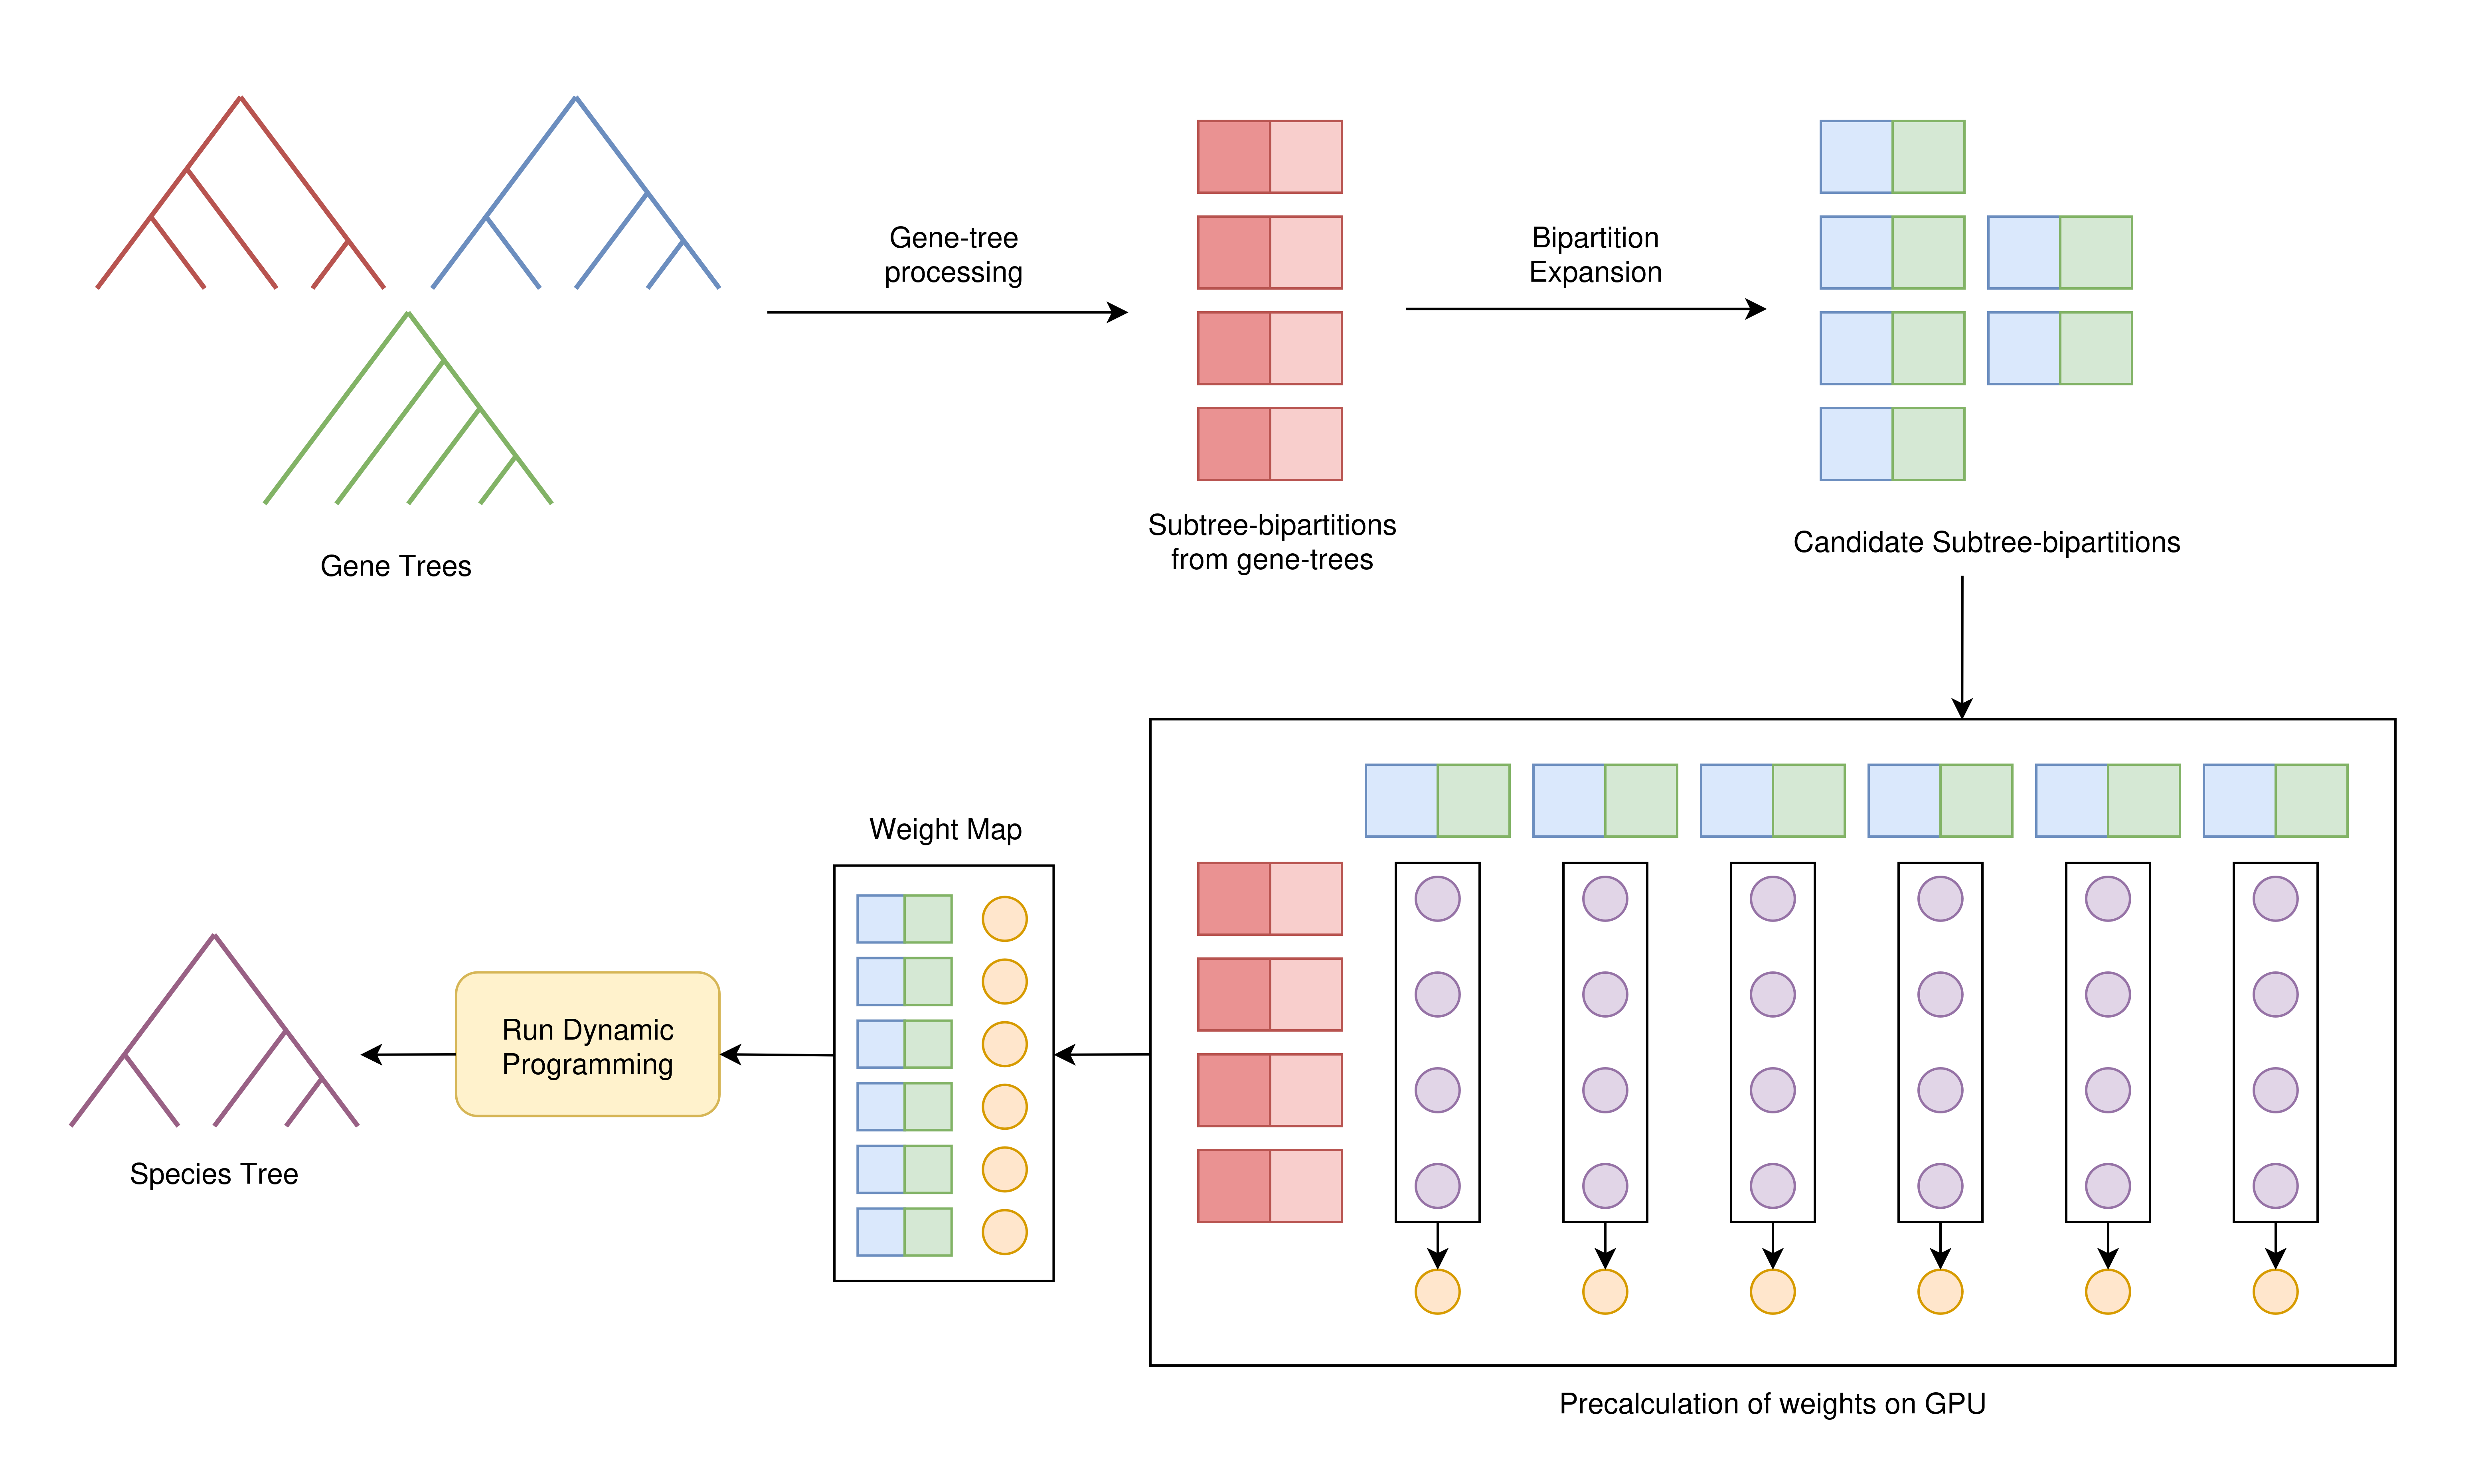
\includegraphics[width=0.9\linewidth]{fig-stx/stelar-flow.png}
    \caption{Algorithmic Framework of STELAR-X Incorporating Dynamic Programming and GPU-Accelerated Weight Mapping}
    \label{fig:stelar-flow}
\end{figure}

\subsection{Formation of Candidate Subtree-Bipartitions}


\subsection{Frequency Mapping of Subtree Bipartitions}

We consider the problem of calculating the frequency of each unique subtree-bipartition in $\mathcal{GB}$ across all gene trees in $\mathcal{G}$. A straightforward approach would be to run a bottom-up dynamic program that represents each subtree-bipartition as a bitset of length $n$, the number of taxa. Using a Hashmap, these bitsets could then be counted to obtain a frequency mapping. However, this approach requires $\mathcal{O}(n^{2}k)$ memory since there are $\mathcal{O}(nk)$ total bipartitions, and each bitset requires $\mathcal{O}(n)$ memory. This quadratic dependence on $n$ makes the method unsuitable for scaling to large numbers of taxa. We therefore propose an alternative representation of subtree-bipartitions that is both memory-efficient and computationally practical.

Consider a gene tree $g_i$, which can be expressed as the post-order traversal of its leaves, yielding a compact array representation $\mathcal{A}_i$. Let $u$ be an internal node in $g_i$ inducing the subtree-bipartition $(A|B)$. By construction, both $A$ and $B$ correspond to contiguous and adjacent subarrays of $\mathcal{A}_i$ because each bipartition corresponds to two contiguous and adjacent post-order intervals. Let $\mathcal{A}_{i,l,r}$ denote the subarray of $\mathcal{A}_i$ from indices $l$ to $r$. Then, if $A = \mathcal{A}_{i,l_1,r_1}$ and $B = \mathcal{A}_{i,l_2,r_2}$, the bipartition $(A|B)$ can be represented as the tuple $(i,l_1,r_1,l_2,r_2)$, where $l_1 < l_2$. In fact, since $l_2 = r_1 + 1$, four integers suffice to store the bipartition. This representation reduces the space requirement from $\mathcal{O}(n^{2}k)$ to $\mathcal{O}(nk)$.

We now focus on the efficient calculation of the frequency mapping under this representation. To do so, we first formalize the notion of equivalence between bipartitions. Let $P$ and $Q$ be sets of taxa. We write $P \sim Q$ if $P$ and $Q$ contain the same taxa, regardless of order. Two subtree-bipartitions $x = (A_1|B_1)$ and $y = (A_2|B_2)$ are said to be equivalent, denoted $x \equiv y$, if either $A_1 \sim A_2$ and $B_1 \sim B_2$, or $A_1 \sim B_2$ and $B_1 \sim A_2$. Thus, equivalence is invariant under permutation of taxa and under swapping of the bipartition sides.

Let $x = (i_x,l_{1x},r_{1x},l_{2x},r_{2x})$ and $y = (i_y,l_{1y},r_{1y},l_{2y},r_{2y})$ be two bipartitions. We distinguish two cases:
\begin{description}
    \item[Case 1: $i_x = i_y$.] Since both bipartitions arise from the same gene tree, their index ranges must either coincide exactly or be disjoint. In fact, two distinct bipartitions of the same tree cannot be equivalent. Therefore, $x \not\equiv y$.
    
    \item[Case 2: $i_x \neq i_y$.] When bipartitions originate from different gene trees, equivalence is possible. A naïve approach would compare the sets of taxa directly, requiring $\mathcal{O}(n)$ time. To avoid this overhead, we employ a hashing-based technique that is both efficient and reliable.
\end{description}

We introduce a permutation-invariant and associative hash function $\phi$ that maps a set of taxa to a hash value independent of ordering. Associativity is essential, as it allows us to use prefix-scan arrays for efficient subarray hashing. Suppose $x \equiv y$. Then, by definition of equivalence, either 
\[
\mathcal{A}_{i_x,l_{1x},r_{1x}} \sim \mathcal{A}_{i_y,l_{1y},r_{1y}} \quad \text{and} \quad \mathcal{A}_{i_x,l_{2x},r_{2x}} \sim \mathcal{A}_{i_y,l_{2y},r_{2y}},
\]
or the same holds with the two sides swapped. Since $\phi$ is permutation-invariant, these relations imply
\[
\phi(\mathcal{A}_{i_x,l_{1x},r_{1x}}) = \phi(\mathcal{A}_{i_y,l_{1y},r_{1y}}) \quad \text{and} \quad \phi(\mathcal{A}_{i_x,l_{2x},r_{2x}}) = \phi(\mathcal{A}_{i_y,l_{2y},r_{2y}}),
\]
or the corresponding equalities under the swap. While equal hash values suggest possible equivalence, hash collisions prevent a strict guarantee. To make the probability of collisions negligible, we employ two safeguards.


First, we adopt double hashing: we use two independent permutation-invariant hash functions, $\phi_1$ and $\phi_2$, and treat the pair $(\phi_1, \phi_2)$ as the final hash signature. Second, we apply an additional single-element hash function $\mathcal{H}$ to taxon identifiers before set-level hashing. Each taxon $t_j \in \mathcal{X}$ is assigned an identifier $d_j \in \{0,1,\ldots,n-1\}$, which is then mapped to a large integer $\mathcal{H}(d_j)$ in a sparse space. For a subarray $\mathcal{A}_{i,l,r}$, we compute
\(
\phi_1(\{\mathcal{H}(d_j)\}_{l \leq j \leq r}), \text{ and } \phi_2(\{\mathcal{H}(d_j)\}_{l \leq j \leq r})
\) for the array $\mathcal{A}_i$.
By leveraging associativity, we precompute prefix-scan arrays for $\phi_1$ and $\phi_2$, which allow subarray hash values to be computed in $\mathcal{O}(1)$ time. All these calculations are performed within the finite field modulo a large prime $P$. Figure~\ref{fig:double-hashing} demonstrates an example of this approach.

\begin{figure}
    \centering
    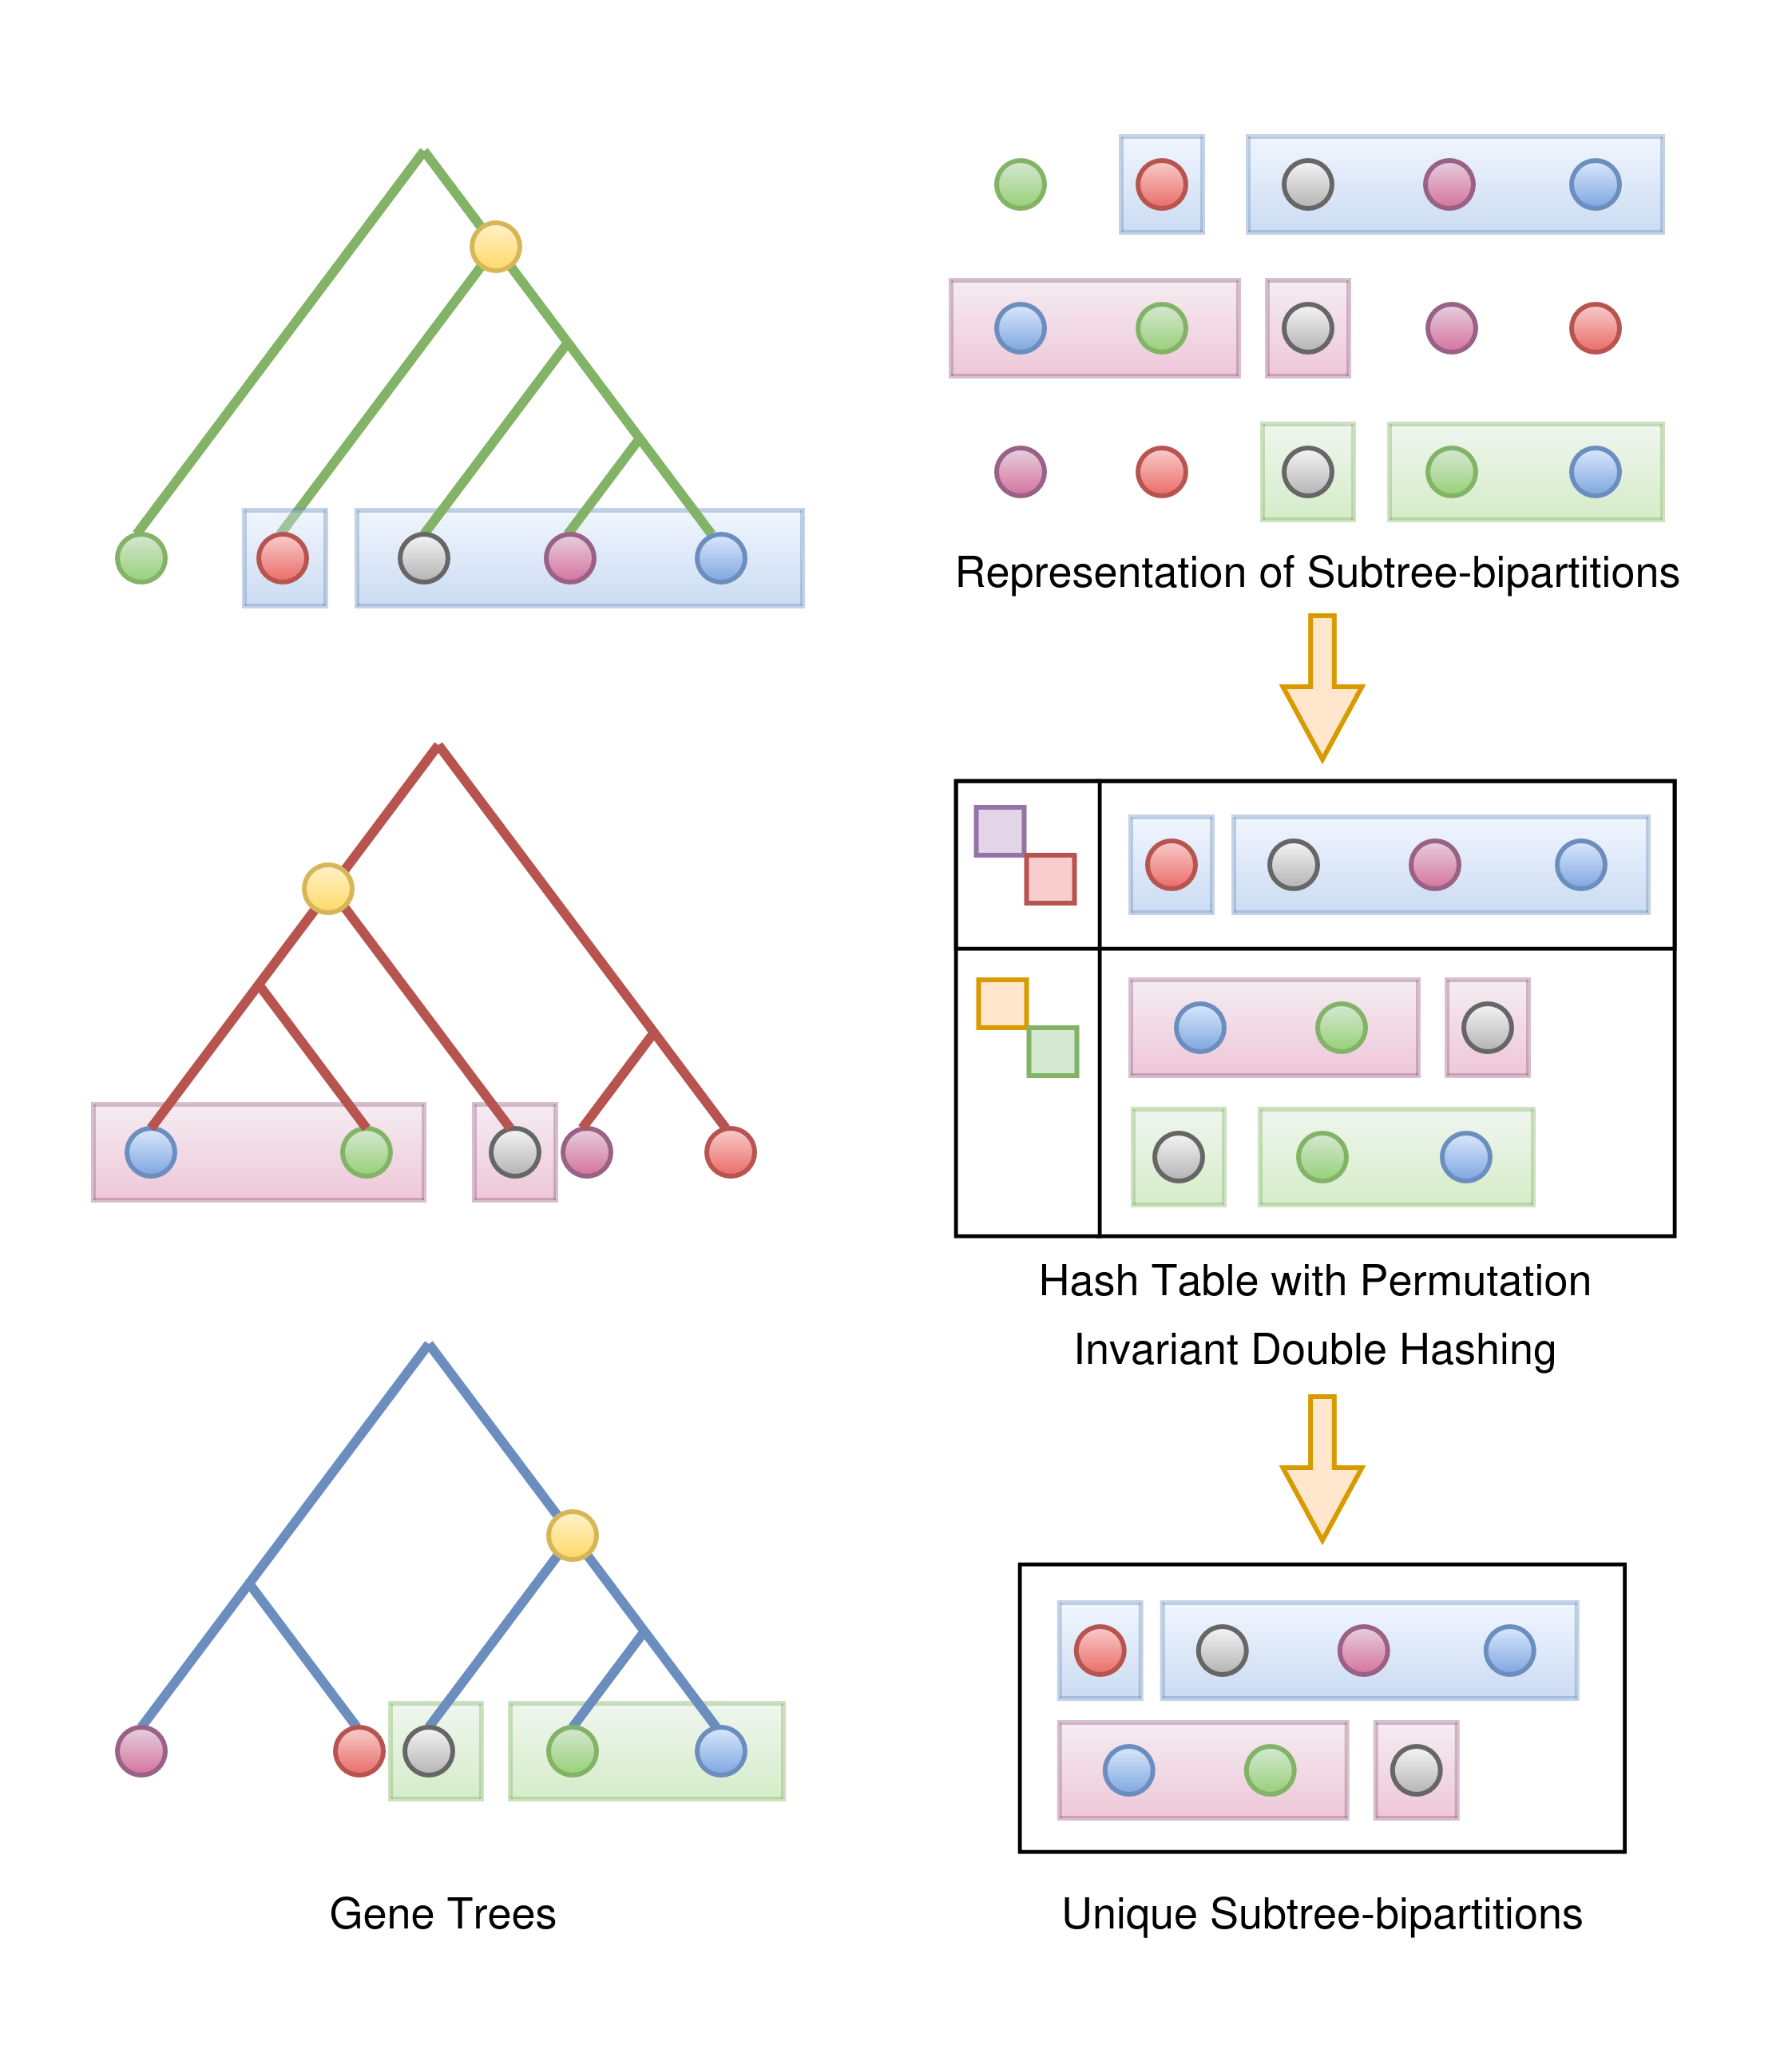
\includegraphics[width=0.5\linewidth]{fig-stx/stelar-diagrams-hashing-unqiue-bips.drawio.png}
    \caption{Determination of unique subtree-bipartitions with permutation-invariant double hashing}
    \label{fig:double-hashing}
\end{figure}

In practice, this combination of double hashing and sparse integer mapping made collisions vanishingly rare. In our implementation, we employ the sum function as $\phi_1$ and the XOR function as $\phi_2$. Across extensive experiments with large datasets, we did not encounter a single collision, demonstrating the robustness of the proposed method.

Finally, we use the hash table to construct a frequency mapping of the unique subtree-biparititions in $\mathcal{O}(\mathcal{|GB|})$ time.








\paragraph{Theoretical Analysis of Collision Probability}  

Now we provide a theoretical analysis of the probability of collisions. The key intuition is that collisions are rare because whenever two sets differ, at least one taxon contributes an independent random value, making accidental equality highly unlikely.

Let $\mathcal{X}$ be the taxon set with $|\mathcal{X}|=n$. Let $M$ be the number of subtree-bipartitions produced across all gene trees (in our setting, $M=\Theta(nk)$). We choose a large prime $P$ and work in the field $\mathbb{F}_P$.

\textbf{Setup.} A single-element hash
\[
\mathcal{H}:\{0,\dots,n-1\}\to\mathbb{F}_P
\]
maps each taxon identifier $d_j$ to
\[
r_j \coloneqq \mathcal{H}(d_j)\in\mathbb{F}_P.
\]
We idealize that the values $\{r_j\}_{j=1}^n$ are independent and uniformly distributed in $\mathbb{F}_P$.

We then apply two associative, permutation-invariant set-level functions $\phi_1,\phi_2$, each operating directly on subsets of $\{r_j\}$. The signature of a set $S$ is
\[
\sigma(S) \coloneqq \big(\phi_1(\{r_j:j\in S\}),\, \phi_2(\{r_j:j\in S\})\big).
\]

\textbf{Single-set collision probability.}  
Let $S\neq T$ and define $U=S\setminus T$, $V=T\setminus S$. Associativity ensures that $\phi_a$ admits a natural cancellation operator $\ominus$ (e.g. subtraction for addition, XOR for XOR, etc.), so that
\[
\phi_a(S)\ominus\phi_a(T) \;=\; \phi_a(U)\ominus\phi_a(V).
\]
Because $U\cup V\neq\varnothing$, at least one $r_t$ appears only in one side. Conditioning on all other $r_j$, the difference reduces to a function of the uniform random variable $r_t$. This equals zero with probability at most $1/P$. Thus
\begin{equation}\label{eq:single-hash}
\Pr\big(\phi_a(S)=\phi_a(T)\big) = \frac{1}{P}.
\end{equation}

\textbf{Pairwise signature collision.}  
Suppose the two set-level functions $\phi_1$ and $\phi_2$ are constructed so that their collision events are statistically independent (e.g.\ by using independent salts or structurally distinct definitions of $\phi_a$). Then for distinct sets $S,T$,
\[
\Pr\big(\sigma(S)=\sigma(T)\big)
= \Pr\big(\phi_1(S)=\phi_1(T)\big)\cdot \Pr\big(\phi_2(S)=\phi_2(T)\big)
= \frac{1}{P^2}.
\]



\textbf{Collision probability for bipartitions.}  
Let bipartitions $x=(A_1 \mid B_1)$ and $y=(A_2 \mid B_2)$ be distinct (non-equivalent).  
A collision occurs if and only if
\[
\big(\sigma(A_1)=\sigma(A_2)\ \wedge\ \sigma(B_1)=\sigma(B_2)\big)
\quad\text{or}\quad
\big(\sigma(A_1)=\sigma(B_2)\ \wedge\ \sigma(B_1)=\sigma(A_2)\big).
\]
Since each matching holds with probability $1/P^2$, we obtain
\[
\Pr\!\big(\text{collision between }x\text{ and }y\big) \;\le\; \frac{2}{P^2}.
\]




\textbf{Global (any-pair) collision probability.}  
Among $M$ bipartitions there are at most $\binom{M}{2}$ pairs. By a union bound,
\[
\Pr(\exists\ \text{collision}) \;\le\; \binom{M}{2}\cdot \frac{2}{P^2}
\;\le\; \frac{M^2}{P^2}.
\]
To keep this probability below a prescribed tolerance $\delta$, it suffices to ensure that
\[
P \;\geq\; \frac{M}{\sqrt{\delta}}.
\]
Hence, choosing $P$ sufficiently larger than $M$ renders global collisions negligible in practice.






\subsection{Precomputation of Bipartition Weights}

We now turn to the theoretical justification for the precomputation of weights associated with all candidate bipartitions in $\mathcal{CB}$. We first explain why these weights are necessary for the dynamic programming (DP) algorithm of STELAR, and then argue that, under the constrained setting, all subtree-bipartitions in $\mathcal{GB}$ must eventually be explored.

Recall that the recursive formulation of STELAR (Equation~\eqref{eq:recurrence-relation}) defines the state space of the DP algorithm. Figure~\ref{fig:stelar-dp} provides an illustration of this state space. Intuitively, the DP begins with a cluster containing all taxa in $\mathcal{X}$. From this initial state, transitions are governed by subtree-bipartitions that partition the taxa of the current cluster. Thus, the evolution of the state space directly depends on the collection of bipartitions available. We now show that, in the constrained version of STELAR, this process inevitably requires the weights of all subtree-bipartitions in $\mathcal{GB}$.

\begin{theorem}
    \label{th:dp-span}
    If $\mathcal{CB} = \mathcal{GB}$, then the state space of the DP algorithm spans every subtree-bipartition $x \in \mathcal{CB}$.
\end{theorem}

\begin{proof}
    We argue by contradiction. Suppose there exists a bipartition $x = (A|B) \in \mathcal{CB}$ that is not explored in the state space of the DP. We consider two possible cases:

    \begin{description}
        \item[Case 1: $A \cup B = \mathcal{X}$]  
        Since $\mathcal{CB} = \mathcal{GB}$, we have $x \in \mathcal{GB}$. As $A \cup B$ covers all taxa, $x$ corresponds to a root-level bipartition in one of the gene trees. By construction, such bipartitions are included in the search space at the very first state transition. This contradicts our assumption that $x$ is not explored.

        \item[Case 2: $A \cup B \neq \mathcal{X}$]  
        Again, $x \in \mathcal{GB}$ and hence arises from some internal node $u$ of a gene tree $g_i$, where the taxa covered by $u$ form the set $\mathcal{Y} = A \cup B$. Since $\mathcal{Y} \subsetneq \mathcal{X}$, $u$ must have a parent node $p$ in $g_i$. Let the bipartition induced by $p$ be $y = (C|D)$. By construction, either $C = \mathcal{Y}$ or $D = \mathcal{Y}$. Thus, if $y$ is explored in the DP state space, then the algorithm must also explore its child bipartition $x$, by design of the transition rules. Hence, the assumption that $x$ is not explored implies that $y$ is also not explored. Repeating this reasoning along the ancestor chain of $u$, we eventually reach the root of $g_i$, where Case~1 applies and yields a contradiction.
    \end{description}

    Since both cases lead to contradictions, our assumption is false. Therefore, every subtree-bipartition $x \in \mathcal{GB}$ is necessarily explored in the constrained DP state space. Thus, precomputing weights is reasonable and justifies isolating this step for GPU acceleration.
\end{proof}

This result shows that, in the constrained setting where $\mathcal{CB} = \mathcal{GB}$, the dynamic programming algorithm must access the weights of all bipartitions in $\mathcal{GB}$. Furthermore, even when $\mathcal{GB} \subsetneq \mathcal{CB}$, as long as $|\mathcal{CB}|$ is not asymptotically larger than $|\mathcal{GB}|$, it remains practical to precompute the weights of all subtree-bipartitions in $\mathcal{CB}$.


We now describe our strategy for precomputing the weights of candidate bipartitions. We begin by recalling the formulation for computing the weight of a single bipartition. Let $x = (A_1|B_1) \in \mathcal{CB}$ denote a candidate subtree-bipartition, and let $y = (A_2|B_2) \in \mathcal{SBP}(g_i)$ be a bipartition in a gene tree $g_i$. It was shown in \cite{Islam-STELAR-2020} that the number of triplets simultaneously mapped to both $x$ and $y$ can be expressed as

\begin{equation}
\mathcal{M}(x,y) = \mathcal{NT}(|A_{1} \cap A_{2}|, |B_{1} \cap B_{2}|) 
+ \mathcal{NT}(|A_{1} \cap B_{2}|, |A_{2} \cap B_{1}|),
\label{eq:Mxy}
\end{equation}

where $\mathcal{NT}(n_1,n_2)$ denotes the total number of triplets mapped to a subtree-bipartition $(A|B)$ of a rooted binary tree, with $|A| = n_1$ and $|B| = n_2$. A straightforward combinatorial argument yields,

\begin{equation}
\mathcal{NT}(n_1, n_2) = \binom{n_1}{2}\binom{n_2}{1} + \binom{n_2}{2}\binom{n_1}{1} 
= \frac{n_1 n_2 (n_1 + n_2 - 2)}{2}.
\label{eq:NT}
\end{equation}

Using these definitions, the weight of bipartition $x$ with respect to the set of gene trees $\mathcal{G}$ can be written as

\begin{equation}
w_{\mathcal{G}}(x) = \sum_{i=1}^{k} \; \sum_{y \in \mathcal{SBP}(g_i)} \mathcal{M}(x,y).
\end{equation}

To reduce computational cost, we take advantage of the frequency mapping of unique subtree-bipartitions obtained earlier. Specifically, let $f_{\mathcal{G}}(y)$ denote the frequency of bipartition $y \in \mathcal{GB}$ across all gene trees in $\mathcal{G}$. Then the weight of $x$ can be equivalently expressed as,

\begin{equation}
w_{\mathcal{G}}(x) = \sum_{y \in \mathcal{GB}} f_{\mathcal{G}}(y)\,\mathcal{M}(x,y).
\label{eq:effcal}
\end{equation}

Equations~\eqref{eq:Mxy} and \eqref{eq:NT} together imply that $\mathcal{M}(x,y)$ can be computed efficiently using bitwise operations on bitsets of length equal to the number of taxa. Once the unique subtree-bipartitions are identified, we encode each of them as a bitset of length $n$, enabling efficient set operations. This representation yields an $\mathcal{O}(n)$ complexity per evaluation, where $n$ is the number of taxa. By Equation~\ref{eq:effcal}, the weight of a single bipartition can thus be computed in $\mathcal{O}(n|\mathcal{GB}|)$ time. Since weights must be computed for all candidate bipartitions $x \in \mathcal{CB}$, the overall cost of precomputation is $\mathcal{O}(n|\mathcal{GB}||\mathcal{CB}|)$.

In the following section, we present strategies for parallelizing the precomputation step, as well as other stages of our algorithm, to further improve scalability.

\subsection{Execution of Dynamic Programming}

As the final step of our algorithm, we execute the dynamic programming procedure using the recursive relation defined in Equation~\eqref{eq:recurrence-relation}. During this execution, an essential requirement is to efficiently identify all subtree-bipartitions $x \in \mathcal{CB}$ that partition the cluster corresponding to the current state.  

To address this, we precompute a map that explicitly defines the state space. Let $x = (A|B) \in \mathcal{CB}$ be a candidate subtree-bipartition. By construction, $x$ partitions the cluster formed by the taxa set $A \cup B$. Accordingly, we define a mapping
\[
\Phi : \{\text{clusters of taxa}\} \;\longrightarrow\; \mathcal{CB},
\qquad 
\Phi(A \cup B) = \{\, x = (A|B) \,\}.
\]
Thus, for each $x \in \mathcal{CB}$, we record its associated cluster $A \cup B$. The algorithm then leverages this precomputed state-space map together with the weight map described earlier to efficiently execute the dynamic programming recurrence. The overall procedure is illustrated in Figure~\ref{fig:stelar-dp}.



\begin{figure}
    \centering
    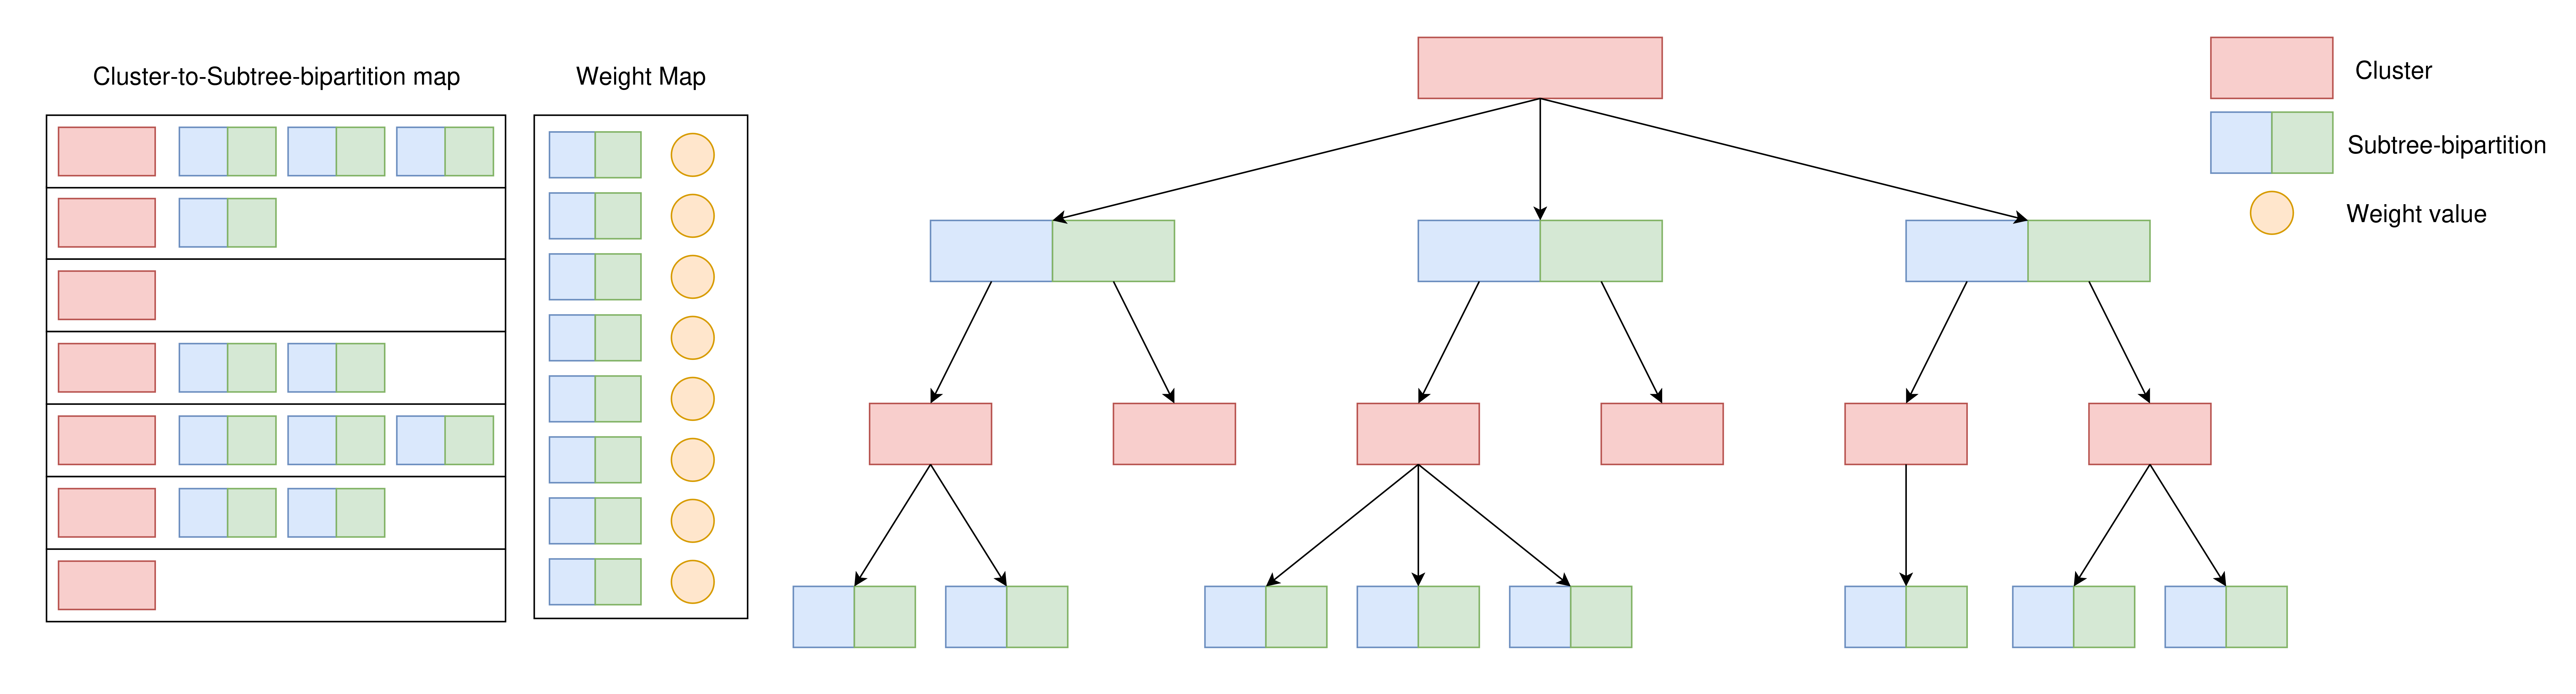
\includegraphics[width=0.9\linewidth]{fig-stx/stelar-algo.png}
    \caption{Dynamic programming algorithm in STELAR-X using cluster-to-subtree-bipartition mapping and precomputed weight mapping}
    \label{fig:stelar-dp}
\end{figure}

\subsection{Parallelization}

We next identify the stages of our algorithm that are amenable to CPU and GPU parallelization. For the complexity analysis, we assume the availability of $T_\mathcal{C}$ CPU threads and $T_\mathcal{G}$ GPU threads that can be executed concurrently. These quantities represent the degree of parallelism achievable under the ideal assumption of perfect load balancing and negligible synchronization or communication overhead. In practice, the actual speedup may be lower; however, this assumption provides a standard theoretical framework for expressing parallel time complexity. 


\subsubsection{CPU Parallelization}

We primarily employ CPU parallelization for parsing and processing the $k$ gene trees. Specifically, the set of gene trees is partitioned into $T_\mathcal{C}$ chunks of approximately equal size, and each chunk is processed in parallel by a separate thread. During the processing of each gene tree, the corresponding frequency mapping is also computed within the same thread. We also employ CPU parallelization while converting the $\mathcal{O}(|\mathcal{GB}|+|\mathcal{CB}|)$ bipartitions into bitsets of length $n$. When necessary, thread-safe data structures and synchronization mechanisms are employed to ensure the correct accumulation of values across threads.


\subsubsection{GPU Parallelization}

We employ GPU acceleration for the precomputation of bipartition weights. As derived earlier, the weight of a single bipartition can be obtained by performing set operations on bitsets of length equal to the number of taxa $n$. To compute the weights for all candidate bipartitions $x \in \mathcal{CB}$, it is therefore necessary to evaluate $\mathcal{M}(x,y)$ for every pair $(x,y)$ where $x \in \mathcal{CB}$ and $y \in \mathcal{GB}$. This corresponds to executing the same operation across $\mathcal{O}(|\mathcal{CB}||\mathcal{GB}|)$ bipartition pairs, followed by accumulation along the $\mathcal{GB}$ dimension to obtain the weights of $\mathcal{O}(|\mathcal{CB}|)$ candidate bipartitions.  

We leverage this highly regular computation pattern to parallelize the precomputation over $T_\mathcal{G}$ GPU threads. In practice, all bipartitions $x \in \mathcal{CB}$ and $y \in \mathcal{GB}$ are encoded as bitsets of length $n$ and transferred to GPU memory, where set operations are performed in parallel. The results are then aggregated to produce a weight map containing $\mathcal{O}(|\mathcal{CB}|)$ entries, which directly feeds into the dynamic programming algorithm. Additional low-level optimizations, such as efficient memory sharing and tiling, are employed to reduce memory latency and further improve throughput.


\subsection{Complexity Analysis}

We now provide a theoretical analysis of the running time and memory requirement of STELAR-X. 

\subsubsection{Running Time Analysis}

The parsing of the $k$ input trees over $T_\mathcal{C}$ CPU threads requires $\mathcal{O}\!\left(\tfrac{nk}{T_\mathcal{C}}\right)$ time. The subsequent computation of the frequency mapping, using the double-hashing approach, also requires $\mathcal{O}\!\left(\tfrac{nk}{T_\mathcal{C}}\right)$ time. This efficiency follows from the use of prefix-scan arrays, which enable constant-time range hash evaluations.  
Next, the conversion of $\mathcal{O}(|\mathcal{GB}|)$ bipartitions from the gene trees and $\mathcal{O}(|\mathcal{CB}|)$ candidate bipartitions into bitset representations requires $\mathcal{O}\!\left(\tfrac{n(|\mathcal{GB}|+|\mathcal{CB}|)}{T_\mathcal{C}}\right)$ time. The precomputation of weights, distributed across $T_\mathcal{G}$ GPU threads, requires $\mathcal{O}\!\left(\tfrac{n|\mathcal{GB}||\mathcal{CB}|}{T_\mathcal{G}}\right)$ time.  

Finally, we analyze the running time of the dynamic programming (DP) algorithm. By Equation~\eqref{eq:recurrence-relation} and Theorem~\ref{th:dp-span}, the size of the DP state space is at most $\mathcal{O}(|\mathcal{CB}|)$. Since both the state-space map and the weight map are precomputed, the DP algorithm itself executes in $\mathcal{O}(|\mathcal{CB}|)$ time.  

Putting all components together, the total running time of our algorithm is
\[
\mathcal{O}\!\left(
\tfrac{nk}{T_\mathcal{C}} \;+\;
\tfrac{n(|\mathcal{GB}|+|\mathcal{CB}|)}{T_\mathcal{C}} \;+\;
\tfrac{n|\mathcal{GB}||\mathcal{CB}|}{T_\mathcal{G}} \;+\;
|\mathcal{CB}|
\right).
\]


\subsubsection{Memory Analysis} 

We now analyze the memory requirements of our algorithm in both CPU RAM and GPU VRAM.  

On the CPU side, storing the $k$ input gene trees over $n$ taxa requires $\mathcal{O}(nk)$ memory. The efficient representation of subtree-bipartitions, together with their subsequent processing, also requires $\mathcal{O}(nk)$ memory. In addition, converting $\mathcal{O}(|\mathcal{GB}|+|\mathcal{CB}|)$ total bipartitions into bitset representations of length $n$ incurs a memory cost of $\mathcal{O}(n(|\mathcal{GB}|+|\mathcal{CB}|))$. The dynamic programming algorithm requires $\mathcal{O}(|\mathcal{CB}|)$ additional space. Overall, the total CPU memory usage is therefore
\[
\mathcal{O}\!\left(nk + n(|\mathcal{GB}|+|\mathcal{CB}|)\right).
\]

On the GPU side, memory usage is dominated by the precomputation of weights. Each bipartition is represented as a bitset of size $n$. Consequently, the total GPU VRAM required for storing all $\mathcal{O}(|\mathcal{GB}|+|\mathcal{CB}|)$ bipartitions is 
\[
\mathcal{O}\!\left(n(|\mathcal{GB}|+|\mathcal{CB}|)\right).
\]





\section{Results}

\subsection{Experimental Setup}

\subsubsection{Datasets}

\subsubsection{Experimental Environment}

\subsection{Accuracy of Inference}

\begin{figure}
    \centering
    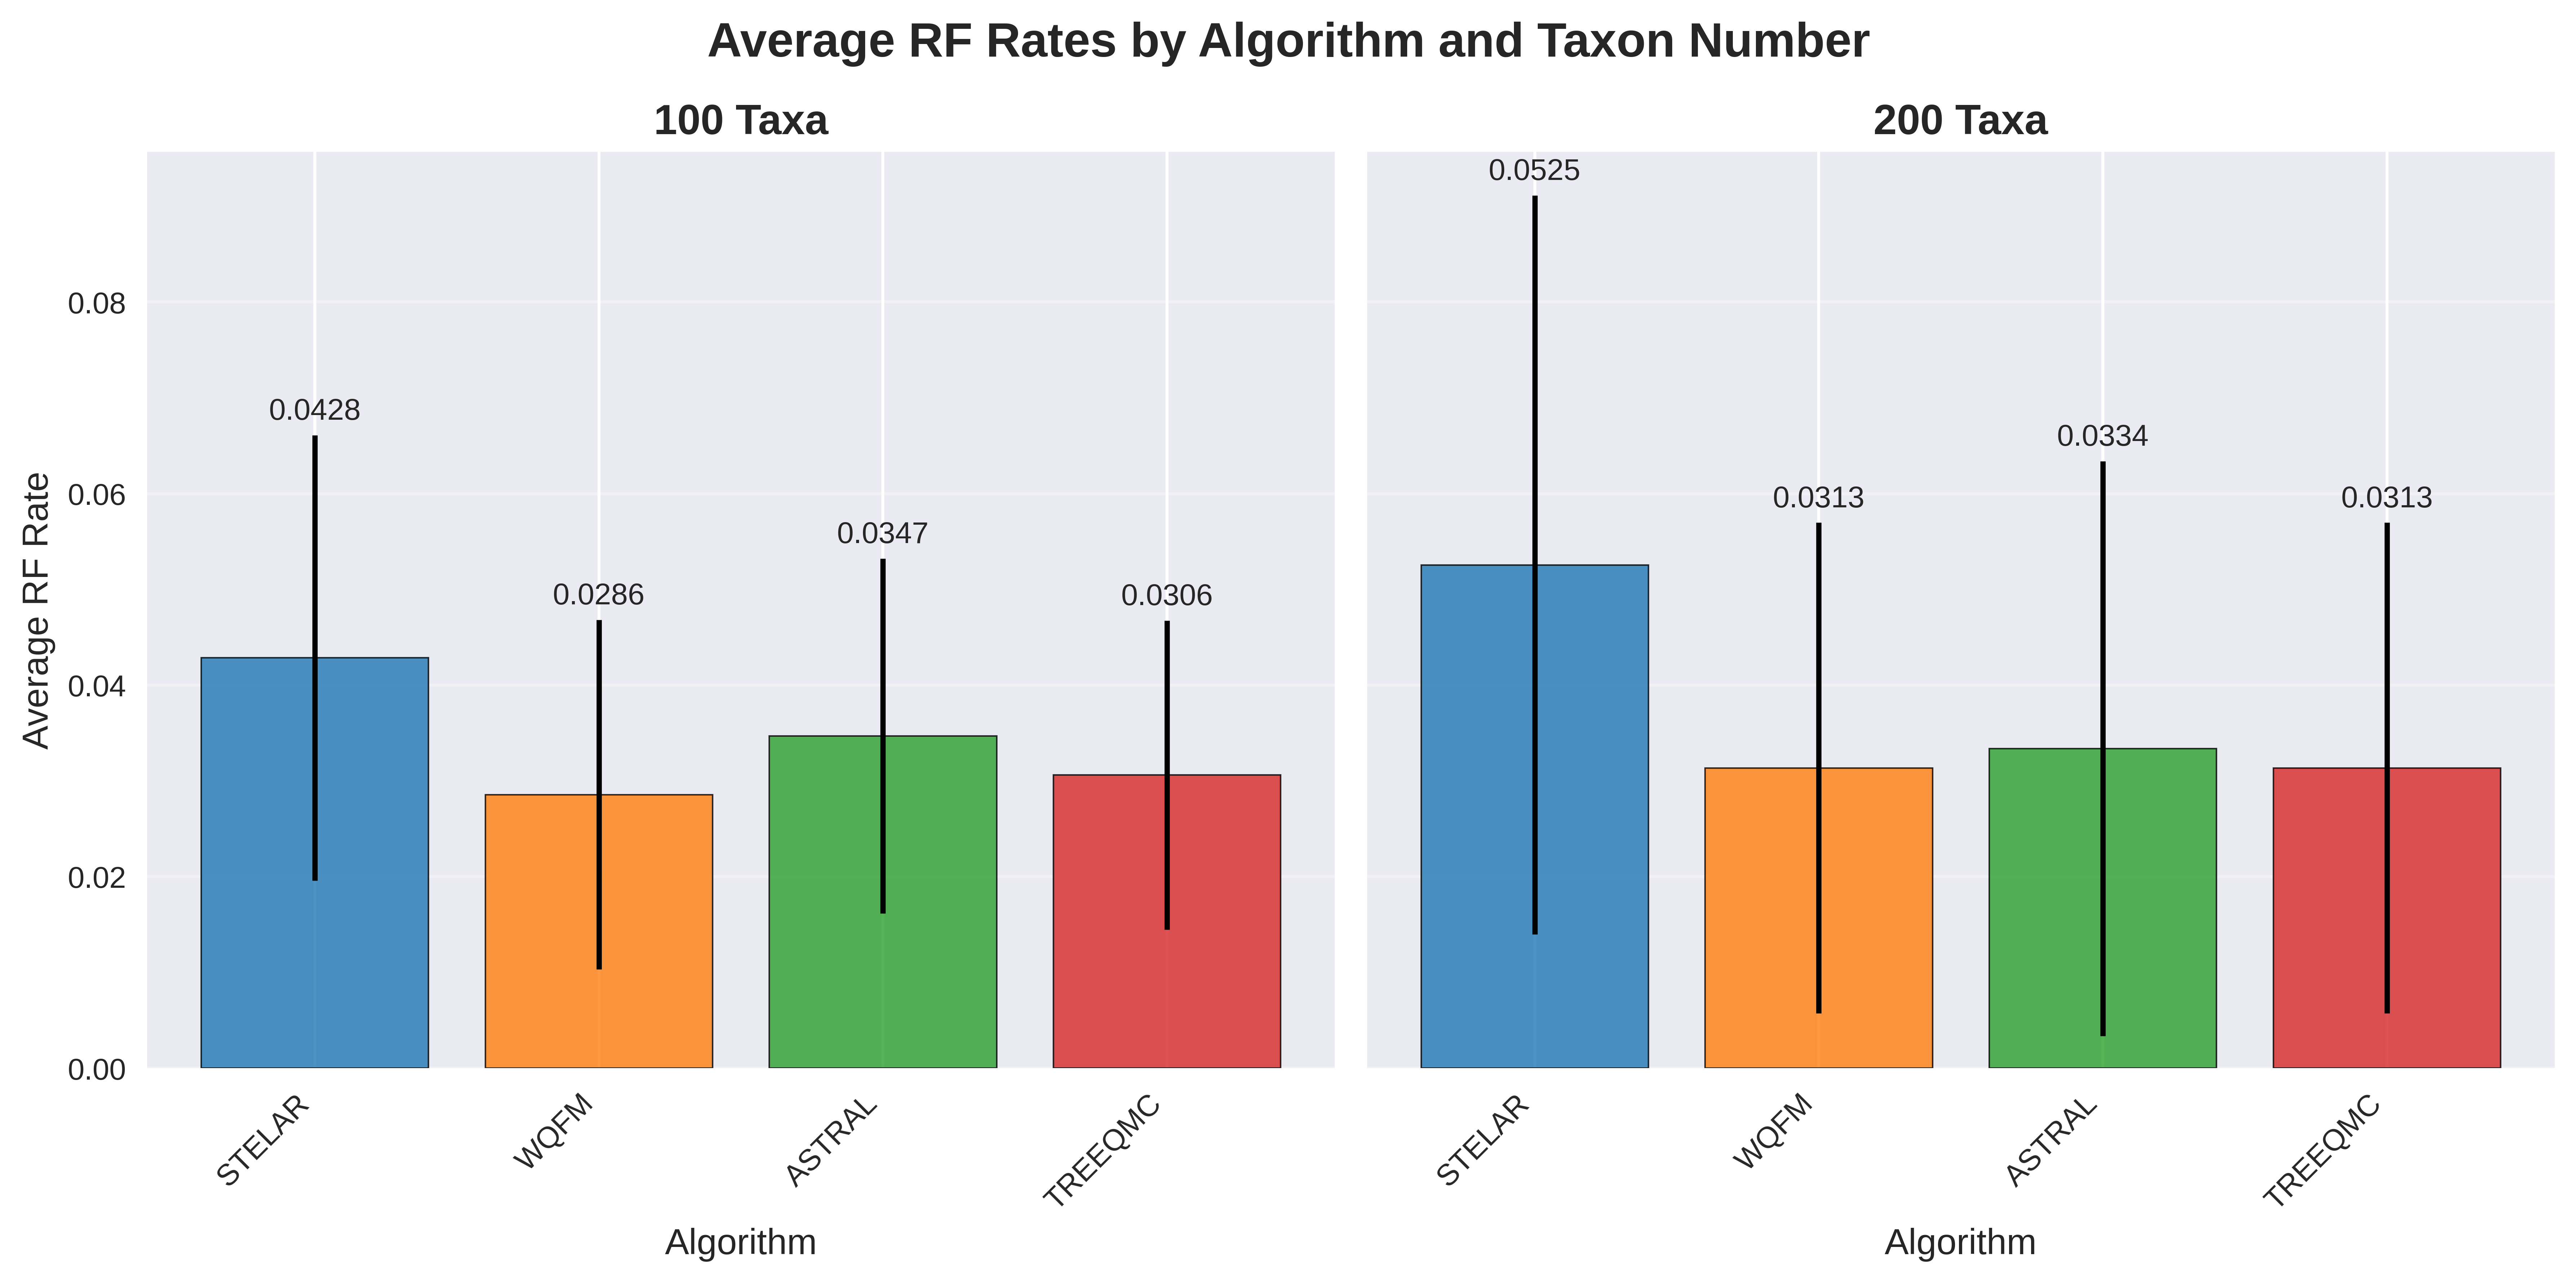
\includegraphics[width=0.8\linewidth]{fig-stx/results/rf_rates_comparison.png}
    \caption{Caption}
    \label{fig:placeholder}
\end{figure}

\subsection{Speedups in Running Time}

\begin{figure}
    \centering
    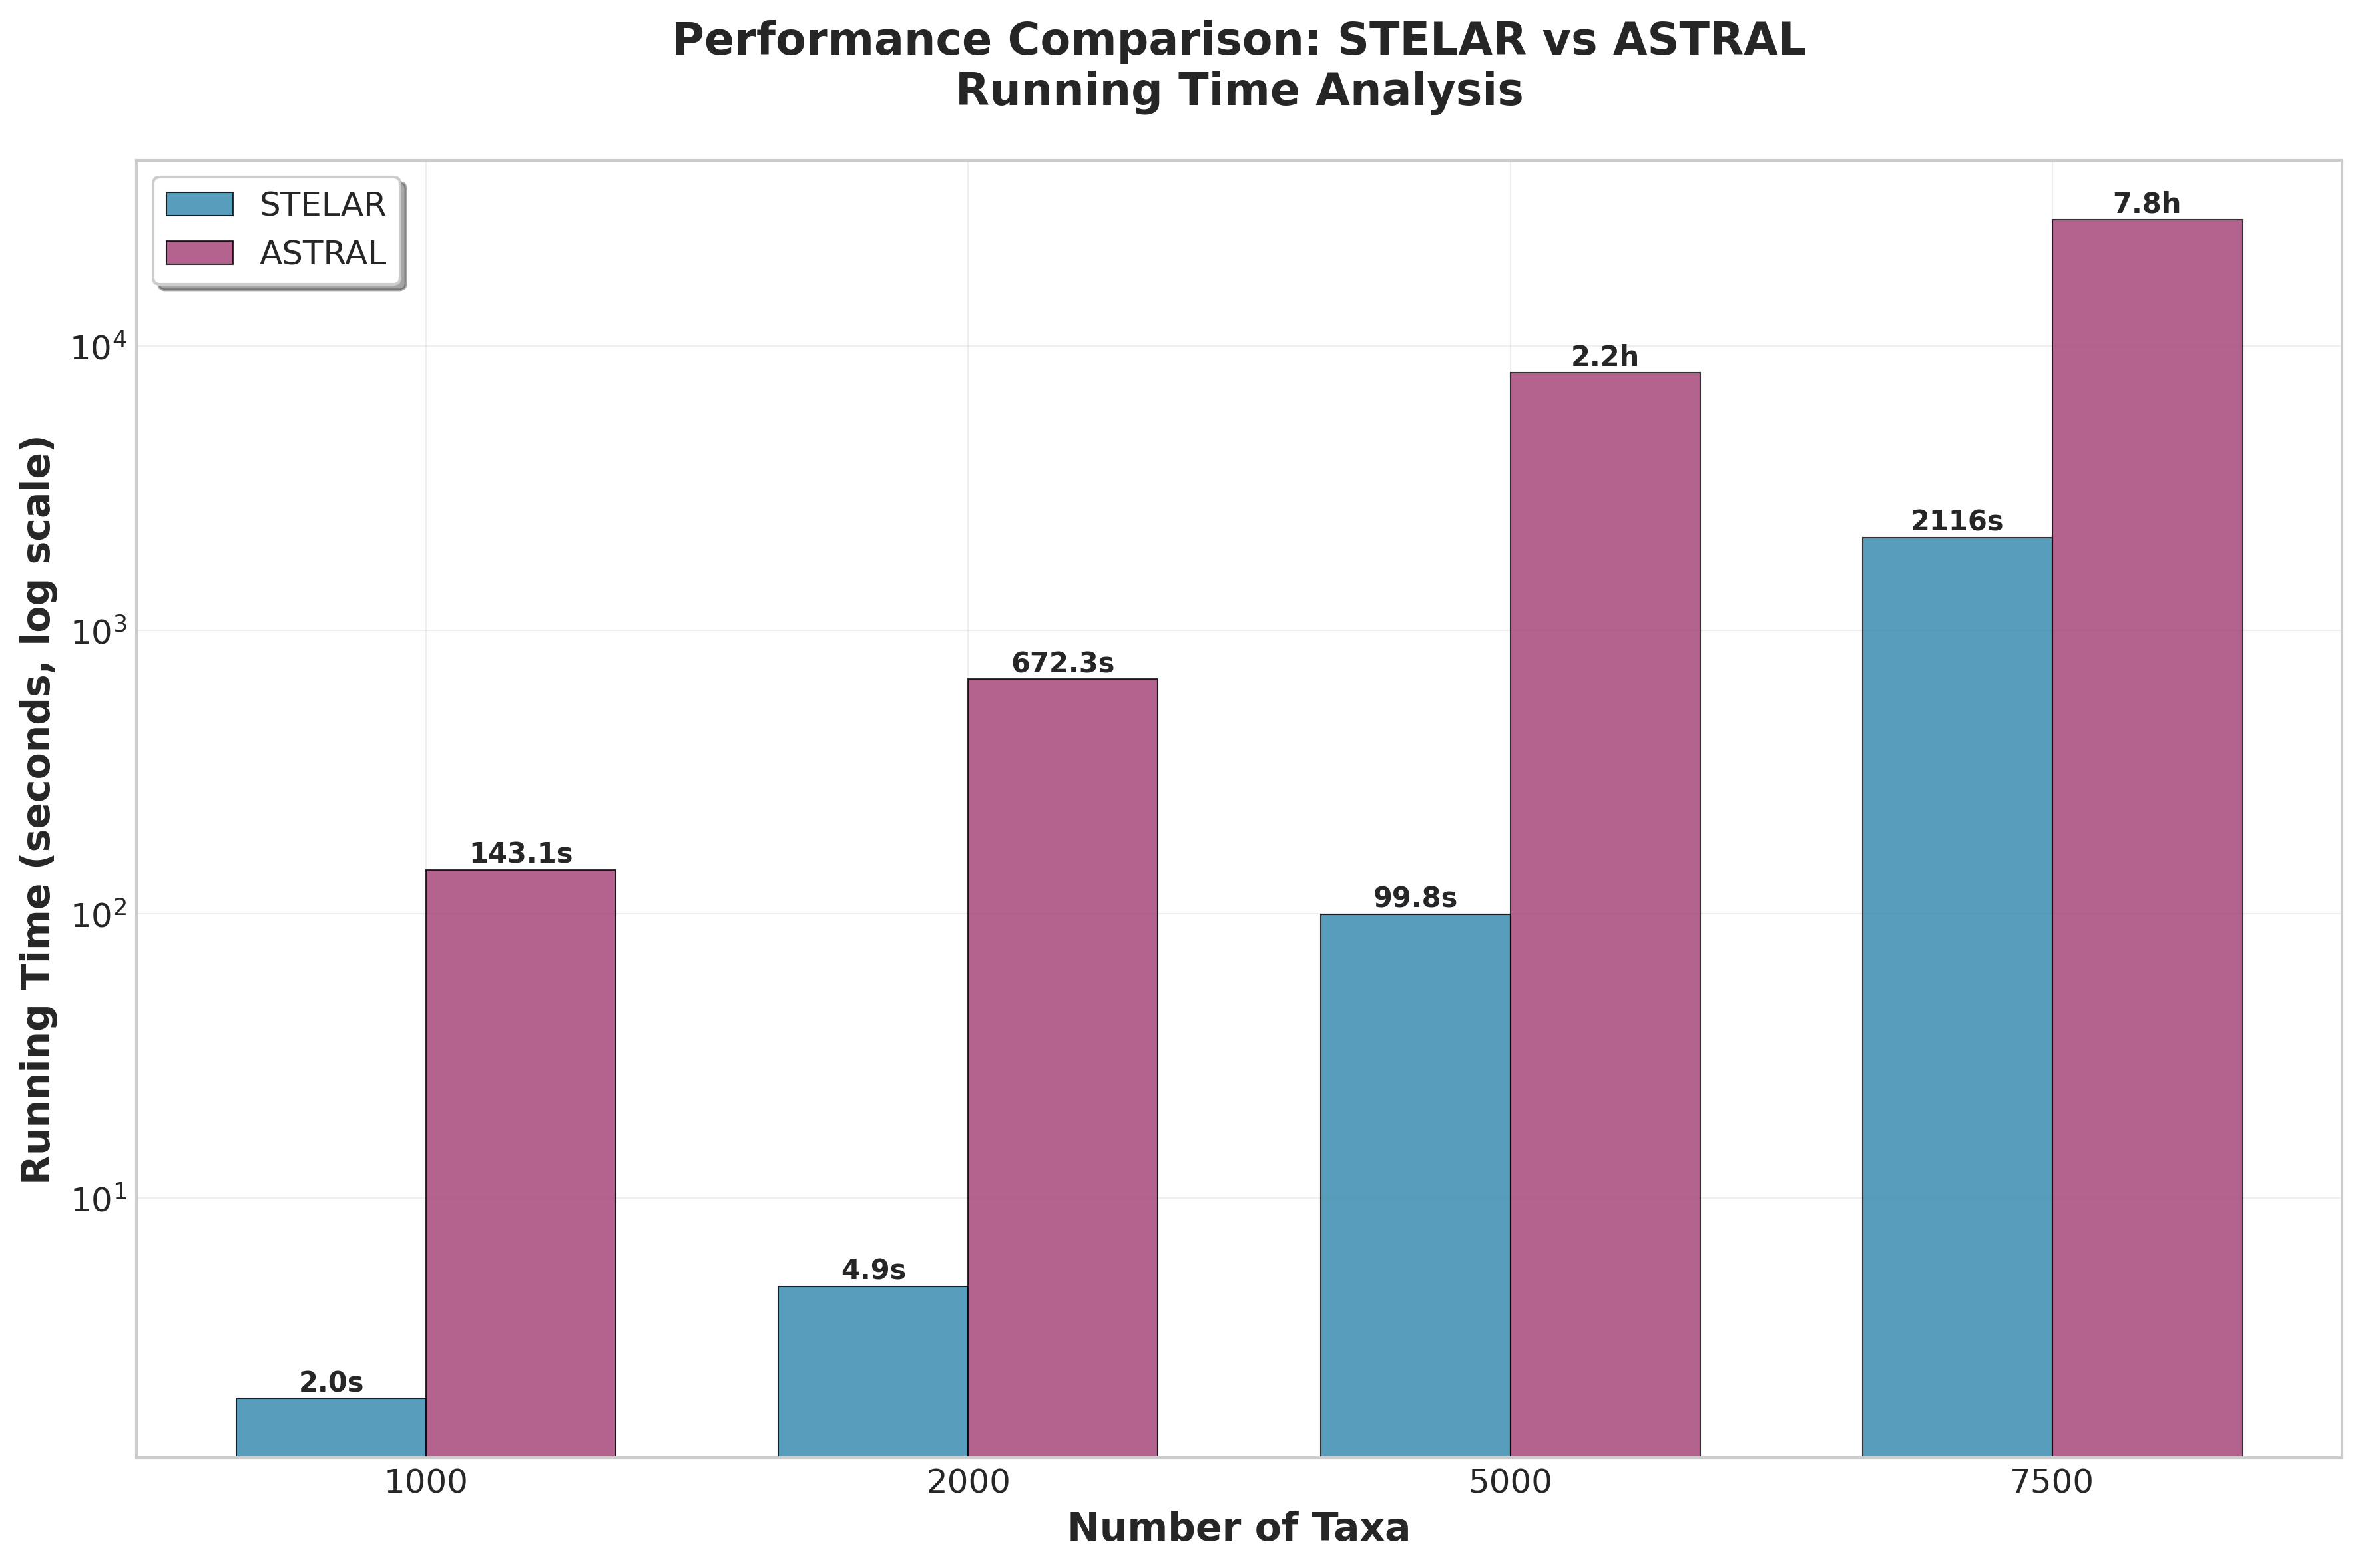
\includegraphics[width=0.5\linewidth]{fig-stx/results/time_comparison.png}
    \caption{Caption}
    \label{fig:placeholder}
\end{figure}

\subsection{Reduction in Memory Usage}

\begin{figure}
    \centering
    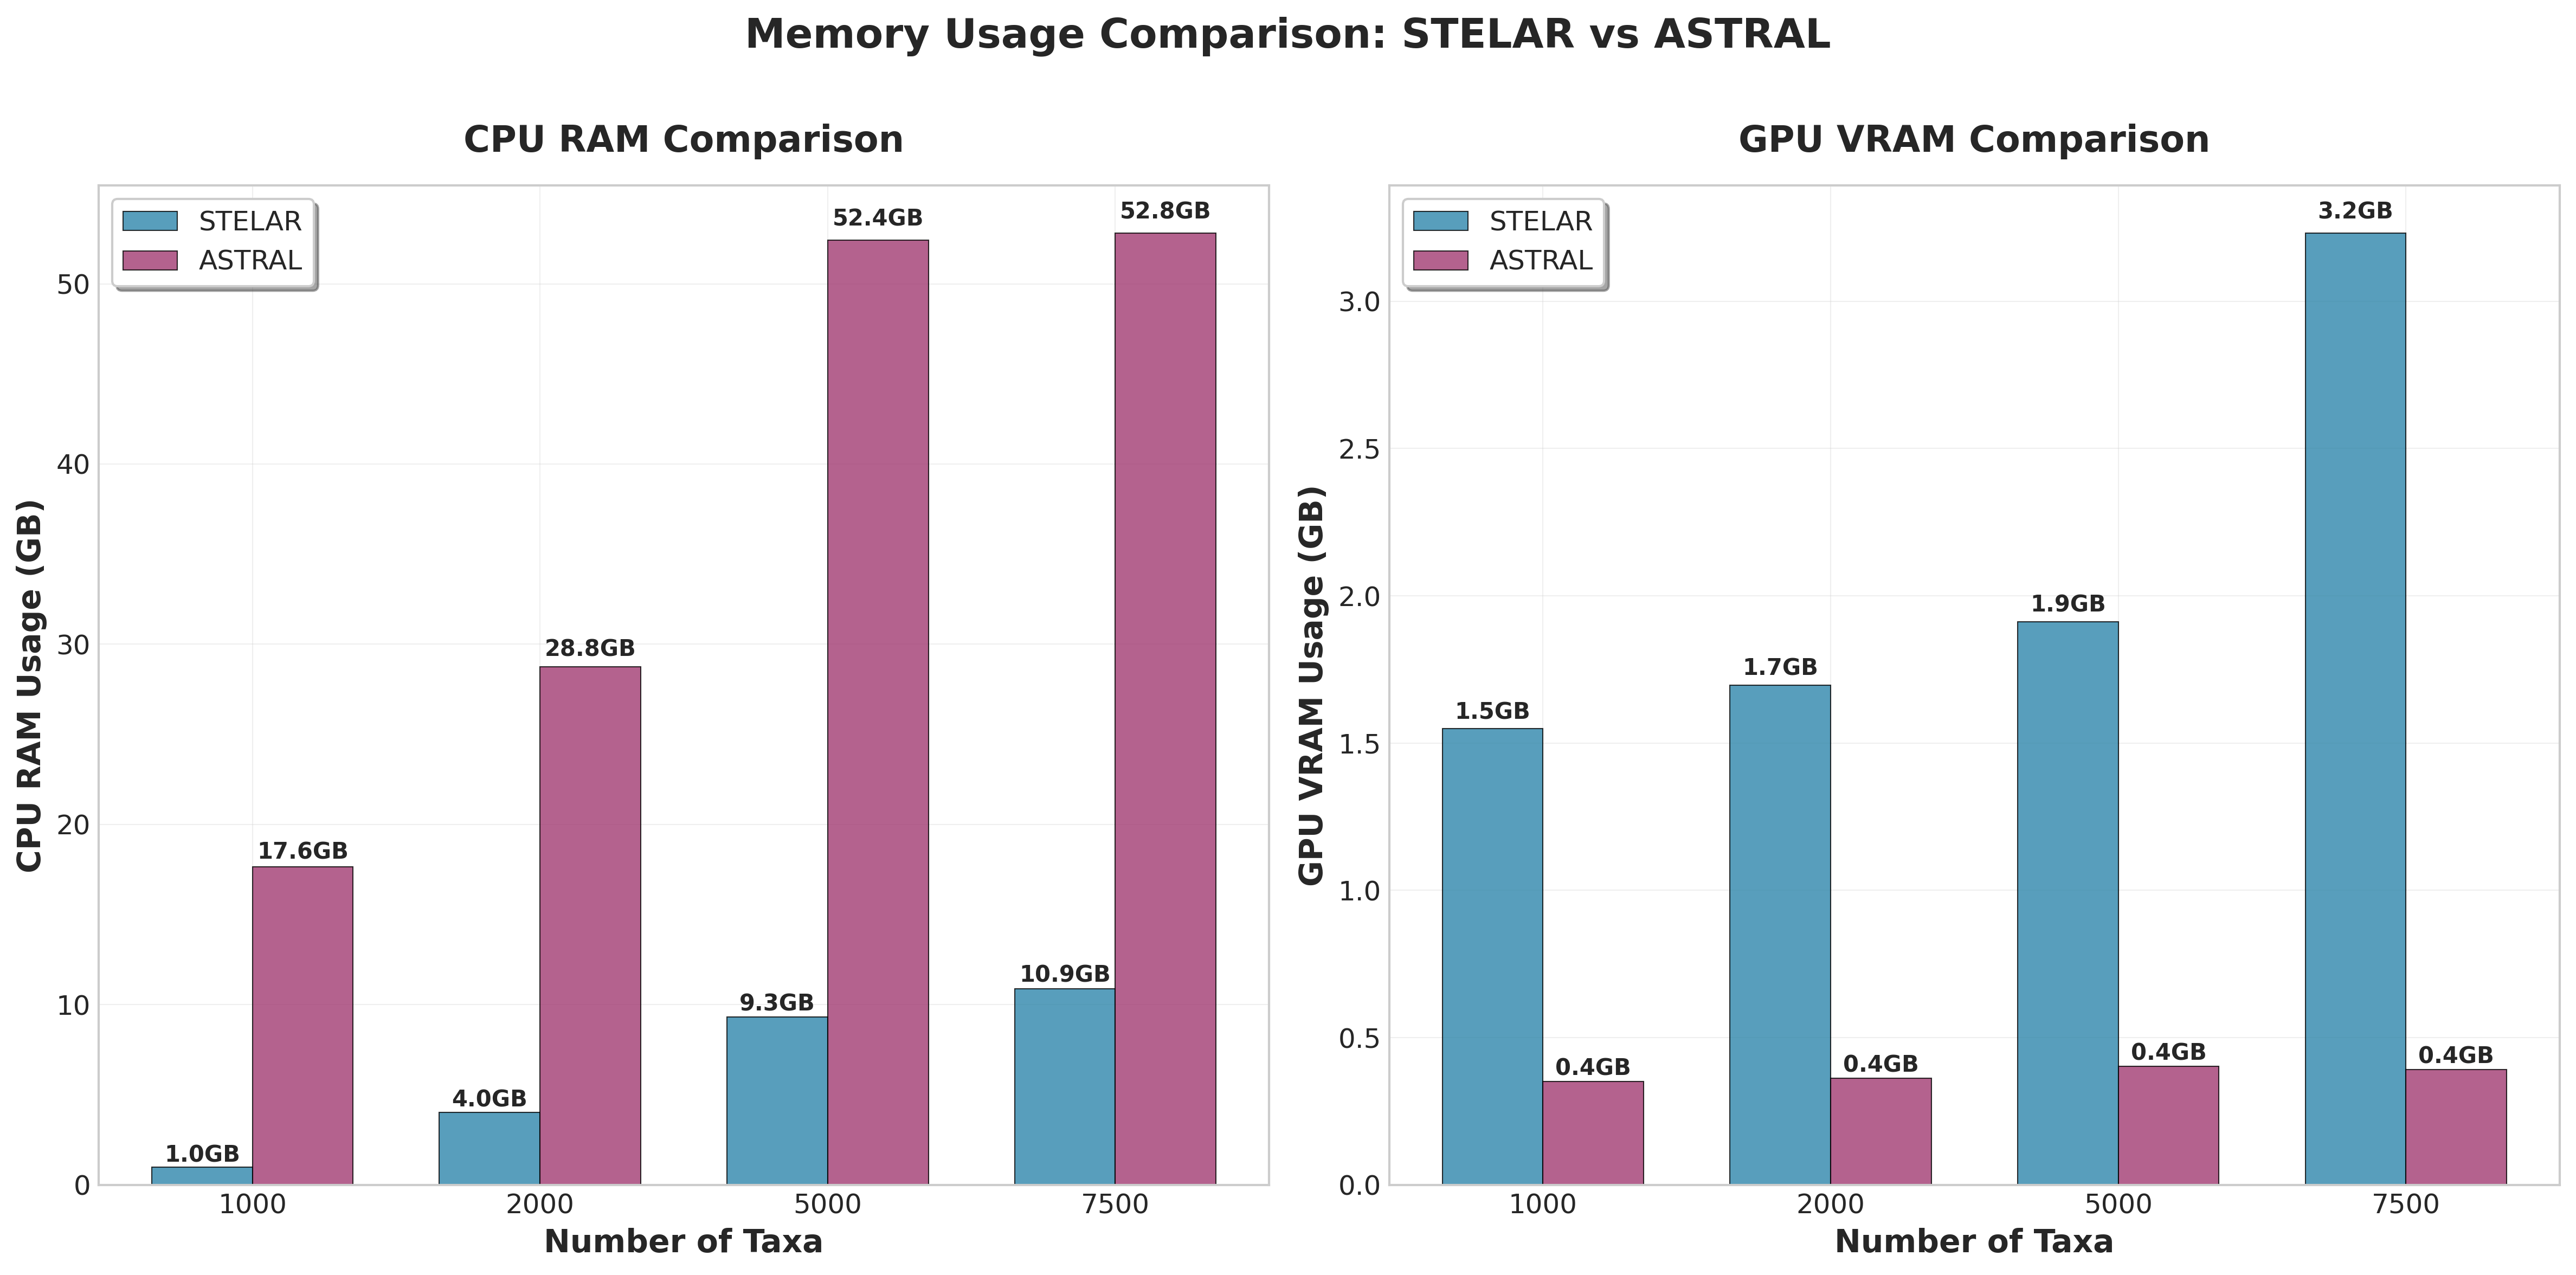
\includegraphics[width=0.9\linewidth]{fig-stx/results/memory_comparison.png}
    \caption{Caption}
    \label{fig:placeholder}
\end{figure}

\subsection{Scaling up the Number of Taxa}

\begin{figure}
    \centering
    
\includegraphics[width=0.9\linewidth]{fig-stx/results/stelar-scale-taxa.png}
    \caption{Caption}
    \label{fig:placeholder}
\end{figure}

\begin{table}[h]
\caption{Running time and memory usage of STELAR with varying number of taxa}
\centering
\begin{tabular}{l l l l l}
\toprule
No. of Taxa & No. of Gene Trees & Running Time (s) & CPU RAM (MB) & GPU VRAM (MB) \\
\midrule
10000  & 1000 & 940.196   & 15499.590 & 2765.824 \\
15000  & 1000 & 2994.442   & 18950.020 & 3941.376 \\
20000  & 1000 & 8141.740   & 27698.211 & 6068.224 \\
25000  & 1000 & 15584.114   & 35323.781 & 8548.352 \\
30000  & 1000 & 27279.418   & 49145.244 & 11340.710 \\
40000  & 1000 & 73897.951   & 71368.128 & 17426.504 \\
50000  & 1000 & 151505.357   & 103244.236 & 27344.662 \\
\bottomrule
\end{tabular}
\end{table}



\subsection{Scaling up the Number of Gene Trees}

\begin{figure}
    \centering
    \includegraphics[width=0.9\linewidth]{fig-stx/results/stelar-scale-gt.png}
    \caption{Caption}
    \label{fig:placeholder}
\end{figure}

\begin{table}[h]
\caption{Running time and memory usage of STELAR with varying number of gene trees}
\centering
\begin{tabular}{l l l l l}
\toprule
No. of Taxa & No. of Gene Trees & Running Time (s) & CPU RAM (MB) & GPU VRAM (MB) \\
\midrule
10000  & 1000 & 940.196   & 15499.590 & 1446.824 \\
10000  & 2500 & 2020.297   & 22062.121 & 1943.992 \\
10000  & 5000 & 3682.449   & 34713.297 & 2458.432 \\
10000  & 7500 & 5259.213   & 48526.764 & 3106.218 \\
10000  & 10000 & 6729.330   & 74323.432 & 3734.514 \\
\bottomrule
\end{tabular}
\end{table}



\section{Discussion}


\section{Conclusion}



\subsection{Datasets}

\subsubsection{Simulated Datasets}

\begin{enumerate}
    \item 100-taxon, 200-taxon -> accuracy comparison among STELAR , ASTRAL, WQFM-TREE, TREE-QMC

    \item Large Simulated Datasets -> accuracy, runtime, CPU RAM, GPU VRAM

    

    
\end{enumerate}

\subsubsection{Empirical Datasets}

\begin{enumerate}
    \item 1kp plant Dataset - accuracy and runtime
\end{enumerate}

\subsection{Simulation Parameters}

\begin{table}[h!]
\centering

\begin{tabular}{|l|l|}
\hline
\textbf{Parameter Name} & \textbf{parameter Value} \\ \hline
\textbf{Speciation rate} & 0.0000001 \\ \hline
Extinsion rate & 0 \\ \hline
Number of Taxa & 100 \\ \hline
Ingroup divergence to the ingroup ratio & 1.0 \\ \hline
Generations & LogN(1.470055e+01,2.500000e-01) \\ \hline
\textbf{Haploid effective population size} & 400000 \\ \hline
Global substitution rate & LogN(-1.727461e+01,6.931472e-01) \\ \hline
Lineage specific rate gamma shape & LogN(1.500000e+00,1) \\ \hline
Gene family specific rate gamma shape & LogN(1.551533e+00,6.931472e-01) \\ \hline
Gene tree branch specific rate gamma shape & LogN(1.500000e+00,1) \\ \hline
Seed & 22 \\ \hline
Sequence Length & 1600 \\ \hline
Sequence base frequencies & Dirichlet(A=36,C=26,G=28,T=32) \\ \hline
Sequence transition rates & Dirichlet(TC=16,TA=3,TG=5,CA=5,CG=6,AG=15) \\ \hline
\end{tabular}
\vspace{6pt}
\caption{Simulation parameters used for the generation of gene trees and species trees in Simphy}
\label{tab:simphy-params}

\end{table}


\section{Results}

% varying num taxa keeping fixed others
% varying num gene trees keeping fixed others


\begin{table}[h]
\caption{Running time comparison of STELAR-X and ASTRAL on large simulated datasets}
\centering
\begin{tabular}{l l l l l l}
\toprule
No. of Taxa & Speciation Rate & Eff. Population Size & No. of Gene Trees & \multicolumn{2}{c}{Running time} \\
 &  &  &  & STELAR-X & ASTRAL \\
\midrule
5000  & 1E-6 & 5e5 & 1000   &    &  \\
     &      & 5e5 & 5000  &    &  \\
     &      & 5e5 & 10000 &     &  \\
10000  & 1E-6 & 5e5 & 1000   &  & \\
     &      & 5e5 & 5000  &  &  \\
     &      & 5e5 & 10000 &  &  \\
20000 & 1E-6 & 5e5 & 500   &    &  \\
     &      & 5e5 & 1000  &     &  \\
     &      & 5e5 & 2000 &    &  \\
30000 & 1E-6 & 5e5 & 500   &    &  \\
     &      & 5e5 & 1000  &     &  \\
     &      & 5e5 & 2000 &    &  \\
\bottomrule
\end{tabular}
\end{table}


\bibliographystyle{splncs04}
\bibliography{ref.bib} 


\end{document}